% Copyright (C) 2007 Technical University of Liberec.  All rights reserved.
%
% Please make a following reference to Flow123d on your project site if you use the program for any purpose,
% especially for academic research:
% Flow123d, Research Centre: Advanced Remedial Technologies, Technical University of Liberec, Czech Republic
%
% This program is free software; you can redistribute it and/or modify it under the terms
% of the GNU General Public License version 3 as published by the Free Software Foundation.
%
% This program is distributed in the hope that it will be useful, but WITHOUT ANY WARRANTY;
% without even the implied warranty of MERCHANTABILITY or FITNESS FOR A PARTICULAR PURPOSE.
% See the GNU General Public License for more details.
%
% You should have received a copy of the GNU General Public License along with this program; if not,
% write to the Free Software Foundation, Inc., 59 Temple Place - Suite 330, Boston, MA 021110-1307, USA.
%
%%%%%%%%%%%%%%%%%%%%%%%%%%%%%%%%%%%%%%%%%%%%%%%%%%%%%%%%%%%%%%%%%%
%
% use PDFLatex to compile this
%

\documentclass[12pt,a4paper]{report}

% our own flow_doc.sty
\usepackage{flow_doc}

\usepackage{listings}
\usepackage{rotating}
\usepackage{pdflscape}
\usepackage{amssymb}
\usepackage{amsmath}
\usepackage{array}
\usepackage{longtable}
\usepackage[usenames,dvipsnames]{color}   %colors
\usepackage{colortbl}   %colorful tables
\usepackage{tabularx}
\usepackage{graphicx} %[dvips]
% it is note used \usepackage{cooltooltips}

%these two can be found in caption package
\usepackage{caption}
\usepackage{subcaption}

\usepackage[numbers]{natbib}

\usepackage{fancyvrb}   % extended verbatim environments (for examples of IO files)

\usepackage{multicol}

\newcommand{\vari}[1]{{\it #1}}
\newcommand{\ditem}[2]{\item[\vari{#1} {\tt #2}]}
\newenvironment{fileformat}{\tt\begin{flushleft}}{\end{flushleft}}
%
%% ini table environment
\newcommand{\key}[1]{{\tt #1 }}
\newcommand{\type}[1]{{\bf #1}}
%
\newenvironment{initable}[1]{%
        \vspace{4ex}
        \noindent
        Section: \textbf{[#1]}\\
        \begingroup
        %%
        %% internal commands of initable environment
        %%
       \newcommand{\br}{\hfill\break}
        %%
        \renewcommand{\arraystretch}{1.4}
        \renewcommand{\tabcolsep}{2mm}
        \small
        \baselineskip 3ex
        %\begin{longtable}{@{}lp{5cm}p{5cm}p{9cm}}%
        \tabularx{\textwidth}{l>{\centering}p{2cm}>{\raggedright}p{2cm}>{\raggedright\arraybackslash}X}%
        %\renewcommand{\\}{\\[3ex]}%
        \hline\hline
        KEY & TYPE & DEFAULT & DESCRIPTION \\%\endhead
        \hline\hline
}{%
        %\end{longtable}
        \endtabularx
        \endgroup
}

%%%%%%%%%%%%%%%%%%%% specific math macros
\def\prtl{\partial}
\def\vc#1{\mathbf{\boldsymbol{#1}}}     % vector
\def\tn#1{{\mathbb{#1}}}    % tensor
\def\abs#1{\lvert#1\rvert}
\def\Abs#1{\bigl\lvert#1\bigr\rvert}
\def\div{{\rm div}}
\def\Lapl{\Delta}
\def\grad{\nabla}
\def\Real{{\mathbf R}}
\def\d {\,{\rm d}}
%% ini_table members


%paths to images
\def\fig{figures}
\def\test_fig{test_graphics}

%%%%%%%%%%%%%%%%%%%%%%%%%%%%%%%%%%%%%%%%%%%%%%%%%%%%%%%%%%%%%%%%%%%%%%%%%%%%%%%%%%%%%%%%%%%%% BEGIN DOCUMENT
%% set specific page layout
\addtolength{\textwidth}{2cm}
\addtolength{\hoffset}{-1.5cm}
\addtolength{\textheight}{4cm}
\addtolength{\voffset}{-2.5cm}
\begin{document}

%%% remove comment delimiter ('%') and select language if required
%\selectlanguage{spanish} 
\thispagestyle{empty}
\begin{center}
\noindent 
\textbf{\LARGE{
  Technical university of Liberec
}}

\vspace{2ex}
\textbf{\LARGE{
  Faculty of mechatronics, informatics\\
  and interdisciplinary studies
}}

\vspace{160pt}

\textbf{\Huge{
Flow123d
}}

\vspace{1cm}
\textbf{\Large{
version 1.8.JHy\_python\_update

}}

\vspace{1cm}

\textbf{\Large{
Documentation of file formats \\
and brief user manual.
}}

\vspace{9cm}




\noindent \textbf{\Large{Liberec, 2015}}

\vspace{1cm}
\pagebreak
\end{center}

\noindent
{\bf Authors:}

\vspace{3ex}    
\noindent
Jan B\v rezina, Jan Stebel, David Flanderka, Pavel Exner, Ji\v r\' i Hn\' idek,

\vspace{3cm}
\noindent
{\bf Acknowledgement}

\vspace{3ex}
\noindent This work was supported by the Ministry of Industry and Trade of the Czech Republic under the project no. FR-TI3/579.

\pagebreak
% \noindent

% \tableofcontents
% \pagebreak
% %\setcounter{page}{2}

% \parindent=0pt
% \parskip=1ex

% \chapter{Getting Started} \label{chapter:getting_started}

% \section{Introduction}
% Flow123D is a software for simulation of water flow, reactionary solute transport and heat transfer in a heterogeneous 
% porous and fractured medium. In particular it is suited for simulation of underground processes in a granite rock massive.
% The program is able to describe explicitly processes in 3D medium, 2D fractures, and 1D channels and exchange between 
% domains of different dimensions. The computational mesh is therefore a collection of tetrahedra, triangles and line segments.

% The water flow model assumes a saturated medium described by the Darcy law. For discretization, we use lumped mixed-hybrid finite element method.
% We support both steady and unsteady water flow. The water flow model can be sequentially coupled with two different models for a solute transport or with a heat transfer model.

% The first solute transport model can deal only with pure advection of several substances without any diffusion-dispersion term. It uses 
% explicit Euler method for time discretization and finite volume method for space discretization and operator splitting method to 
% couple with various processes described by the reaction term. The reaction term can treat any meaningful combination of the dual porosity, sorptions, decays and linear reactions.
% Alternatively, one can use interface to the experimental SEMCHEM package for more complex geochemistry.

% The second solute transport model describes general advection with hydrodynamic dispersion for several substances. It uses implicit Euler method for time discretization and discontinuous Galerkin method of
% the first, second or third order for the discretization in space. Currently there is no support for reaction term, the operator splitting approach (although it is not suited for implicit time schemes) 
% is planned for the next version.

% The heat transfer model assumes equilibrium between temperature of the rock and the fluid phase. It uses the same numerical scheme as the second transport model.

% The program support output of all input and many output fields into two file formats. You can use file format of GMSH mesh generator and post-processor 
% or you can use output into widely supported VTK format. In particular we recommend Paraview software for visualization and post-processing of the VTK data.

% The program is implemented in C/C++ using essentially PETSC library for linear algebra. All models can run in parallel using MPI environment, however, 
% the scalability of the whole program is limited due to serial mesh and serial outputs.


% The program is distributed under GNU GPL v. 3 license and is available on the project web page:
% \url{http://flow123d.github.io}

% with sources on the GitHub:
% \url{https://github.com/flow123d/flow123d}.


% \section{Reading Documentation}
% The Flow123d documentation has two main parts. The first three chapters form a user manual which
% starts with getting and running the program and tutorial problem in chapter \ref{chapter:getting_started}. 
% The second chapter \ref{chapter:mathematical_models} provides detailed description of mathematical models
% of physical reality. The third chapter \ref{chapter:file-formats} documents all file types used by Flow123d, 
% including mesh files, input and output files.

% The second main part, consisting only of the chapter \ref{chapter:input-tree-reference}, is automatically
% generated. It mirrors directly the code and contains the whole input tree of the main input file. Description
% of input records, their structure and default values are supplied there and bidirectional links to the user 
% manual are provided.


% \section{Running Flow123d}
% On the Linux system the program can be started either directly or through a script \verb'flow123d.sh', both placed in the \verb'bin' directory of the installation 
% package or of the source tree. When started directly, e.g. by the command
% \begin{verbatim}
%   > flow123d -s example.con
% \end{verbatim}
% the program requires one argument after switch \verb'-s' which is the name of the principal input file. Full list of possible command line arguments is as follows.

% %  --help                  produce help message
% %  -s [ --solve ] arg      Main input file to solve.
% %  -i [ --input_dir ] arg  Directory for the ${INPUT} placeholder in the main 
% %                          input file.
% %  -o [ --output_dir ] arg Directory for all produced output files.
% %  -l [ --log ] arg        Set base name for log files.
% %  --no_log                Turn off logging.
% %  --no_profiler           Turn off profiler output.
% %  --full_doc              Prints full structure of the main input file.
% %  --JSON_template         Prints description of the main input file as a valid 
% %                          CON file.
% %  --latex_doc             Prints description of the main input file in Latex 
% %                          format using particular macros.


% \begin{description}
%  \item[{\tt --help}] \hfill\\
%         Parameters interpreted by Flow123d. Remaining parameters are passed to PETSC.
%  \item[ {\tt -s, --solve} ] \verb'<file>' \hfill\\
%  	 Set principal CON input file. All relative paths in the CON file are relative against current directory.
%  \item[{\tt -i, --input\_dir}] \verb'<directory>' \hfill\\
%  	The placeholder \verb"${INPUT}" %$
%   	used in the path of an input file will be replaced by the \verb'<directory>'. Default value is \verb'input'.
%  \item[{\tt -o, --output\_dir}] \verb'<directory>' \hfill\\
%  	All paths for output files will be relative to this \verb'<directory>'. Default value is \verb'output'.
%  \item[{\tt -l, --log}] \verb'<file_name>' \hfill\\
%  	Set base name of log files. Default value is \verb'flow123d'. The log files are individual for every MPI process, placed in the output directory. 
%  	The MPI rank of the process and the \verb'log' suffix are appended to the base name.
%  \item[{\tt --no\_log}] \hfill\\
%         Turn off logging.
%  \item[{\tt --no\_profiler}] \hfill\\
%         Turn off profiler output.
%  \item[{\tt --full\_doc}] \hfill\\
%         Prints full structure of the main input file.
%  \item[{\tt --markdown_example\_doc}] \hfill\\
%         Prints a description of the main input file in LaTeX format using particular macros.
% \end{description}
% All other parameters will be passed to the PETSC library. An advanced user can influence lot of parameters of linear solvers. In order to get list of supported options 
% use parameter \verb'-help' together with some valid input. Options for various PETSC modules are displayed when the module is used for the first time.


% Alternatively, you can use script \verb'flow123d.sh' to start parallel jobs or limit resources used by the program. 
% The syntax is as follows:

% \begin{verbatim}
%   flow123d.sh [OPTIONS] -- [FLOW_PARAMS]
% \end{verbatim}
% where everything after double dash is passed as parameters to the flow123d binary. The script accepts following options:

% \begin{description}
%   \item[{\tt -h, --help}] \hfill\\
%   	Usage overview.
%   \item[{\tt --host}] \verb'<hostname>' \hfill\\
%         Default value is the host name obtained by system \verb'hostname' command, this argument can be used to override it. 
%         Resulting value is used to select a backend script \verb'config/<hostname>.sh', which describes particular method how to start 
%         parallel jobs, usually through some sort of PBS job queue system. If the script is not found, we try to start parallel processes 
%         directly on the actual host."
%   \item[{\tt -t, --walltime}] \verb'<timeout>' \hfill\\
%   	Upper estimate for real running time of the calculation. Kill calculation after {\it timeout} seconds. 
%   	Can also be used by PBS to choose appropriate job queue. 
%   \item[{\tt -np}] \verb'<number of processes>' \hfill\\
%   	Specify number of MPI parallel processes for calculation.
%   \item[{\tt -m, --mem}] \verb'<memory limit>' \hfill\\
%   	Limits total available memory to \verb'<memory limit>' bytes per process.
%   \item[{\tt -n, --nice}] \verb'<niceness>' \hfill\\
%   	Change priority of the calculation, higher values means lower priority. See the {\tt nice} command.
%   \item[{\tt -ppn}] \verb'<processes per node>' \hfill\\
%        Set number of processes started on one node for multicore systems. 
%        Number of processes set by \verb'-np' parameter should be divisible by \verb'<processes per node>'.
%   \item[{\tt -q, --queue}] \verb'<queue>' \hfill\\
%        Select particular job queue on PBS systems. If running without PBS, 
%        it redirects stdout and stderr to the file \verb'<queue>.<date>', which appended date and time of the start of the job.
% \end{description}

% On the windows operating systems, we use Cygwin libraries in order to emulate Linux API.
% Therefore you have to keep the Cygwin libraries within the same directory as the program executable.
% The Windows package that can be downloaded from project web page contains both the Cygwin libraries
% and the mpiexec command for starting parallel jobs on the windows based workstations.

% Then you can start the sequential run by the command:
% \begin{verbatim}
%   > flow123d.exe -s example.con
% \end{verbatim}
% or the parallel run by the command:
% \begin{verbatim}
%   > mpiexec.exe -np 2 flow123d.exe -s example.con
% \end{verbatim}
% The program accepts the same parameters as the Linux version, but there is no script similar to \verb'flow123d.sh' for the windows operating systems.




% 

\section{Tutorial Problem}
In the following section, we shall provide an example cook book for preparing and running a model. It is 
one of the test problem with the main input file:
\begin{verbatim}
tests/03_transport_small_12d/flow_vtk.con
\end{verbatim}
We shall start with preparation of the geometry using an external software and then we shall go thoroughly through the 
commented main input file. The problem includes steady Darcy flow, transport of two substances with explicit
time discretization and a reaction term consisting of dual porosity and sorption model.

\subsection{Geometry}
We consider a~simple 2D problem with a branching 1D fracture (see Figure \ref{fig:tutorial} for the geometry). 
To prepare a~mesh file we use the \href{http://geuz.org/gmsh/}{GMSH software}.
First, we construct a~geometry file. In our case the geometry consists of: 
\begin{itemize}
 \item one physical 2D domain corresponding to the whole square
 \item three 1D physical domains of the fracture
 \item four 1D boundary physical domains of the 2D domain
 \item three 0D boundary physical domains of the 1D domain
\end{itemize}
In this simple example, we can in fact combine physical domains in every group, however we use this more complex setting for
demonstration purposes. Using GMSH graphical interface we can prepare the GEO file where physical domains are referenced by numbers, then we use 
any text editor and replace numbers with string labels in such a way that the labels of boundary physical domains start with the dot character. 
These are the domains where we will not do any calculations but we will use them for setting boundary conditions.
Finally, we get the GEO file like this:

\begin{multicols}{2}
{\small
\begin{Verbatim}[numbers=left]
cl1 = 0.16;
Point(1) = {0, 1, 0, cl1};
Point(2) = {1, 1, 0, cl1};
Point(3) = {1, 0, 0, cl1};
Point(4) = {0, 0, 0, cl1};
Point(6) = {0.25, -0, 0, cl1};
Point(7) = {0, 0.25, 0, cl1};
Point(8) = {0.5, 0.5, -0, cl1};
Point(9) = {0.75, 1, 0, cl1};
Line(19) = {9, 8};
Line(20) = {7, 8};
Line(21) = {8, 6};
Line(22) = {2, 3};
Line(23) = {2, 9};
Line(24) = {9, 1};
Line(25) = {1, 7};
Line(26) = {7, 4};
Line(27) = {4, 6};
Line(28) = {6, 3};
\end{Verbatim}
\columnbreak
\begin{Verbatim}[numbers=left, firstnumber=last]
Line Loop(30) = {20, -19, 24, 25};
Plane Surface(30) = {30};
Line Loop(32) = {23, 19, 21, 28, -22};
Plane Surface(32) = {32};
Line Loop(34) = {26, 27, -21, -20};
Plane Surface(34) = {34};
Physical Point(".1d_top") = {9};
Physical Point(".1d_left") = {7};
Physical Point(".1d_bottom") = {6};
Physical Line("1d_upper") = {19};
Physical Line("1d_lower") = {21};
Physical Line("1d_left_branch") = {20};
Physical Line(".2d_top") = {23, 24};
Physical Line(".2d_right") = {22};
Physical Line(".2d_bottom") = {27, 28};
Physical Line(".2d_left") = {25, 26};
Physical Surface("2d") = {30, 32, 34};
\end{Verbatim}
}
\end{multicols}

Notice the labeled physical domains on lines 26 -- 36. Then we just set the discretization step \verb'cl1' and use GMSH to create the mesh file.
The mesh file contains both the 'bulk' elements where we perform calculations and the 'boundary' elements (on the boundary physical domains) where we only set the boundary conditions.

\subsection{CON File Format}
The main input file uses a slightly extended JSON file format which together with some particular constructs forms a CON (C++ object notation) file format. 
Main extensions of the JSON are unquoted key names (as long as they do not contain whitespaces), possibility to use \verb'=' instead of \verb':' 
and C++ comments, i.e. \verb'//' for a one line and \verb'/* */' for a multi-line comment. In CON file format, we prefer to call JSON objects ``records'' and we introduce also ``abstract records''
that mimic C++ abstract classes, arrays of a CON file have only elements of the same type (possibly using abstract record types for polymorphism). 
The usual keys are in lower case and without spaces (using underscores instead),
there are few special upper case keys that are interpreted by the reader: \verb'REF' key for references, \verb'TYPE' key for specifing actual type of an abstract record.
For detailed description see Section \ref{sec:CONformat}.


Having the computational mesh from the previous step, we can create the main input file with the description of our problem. 
\begin{Verbatim}[numbers=left]
{
  problem = {
    TYPE = "SequentialCoupling", 
    description = "Tutorial problem: 
    Transport 1D-2D (convection, dual porosity, sorption, sources).", 
    mesh = {
      mesh_file = "./input/mesh_with_boundary.msh",
      sets = [
          { name="1d_domain", 
            region_labels = [ "1d_upper", "1d_lower", "1d_left_branch" ]
          }
        ]
    }, // mesh
\end{Verbatim}
The file starts with a selection of problem type (\verb'SequentialCoupling'), and a textual problem description.
Next, we specify the computational mesh, here it consists of the name of the mesh file and the declaration of one {\it region set} 
composed of all 1D regions i.e. representing the whole fracture. Other keys of the \hyperlink{IT::Mesh}{\tt mesh} record allow labeling regions given only by numbers, 
defining new regions in terms of element numbers (e.g to have leakage on single element), 
defining boundary regions, and set operations with region sets, see Section \ref{sec:Mesh} for details.

\subsection{Flow Setting}
Next, we setup the flow problem. We shall consider a flow driven only by the pressure gradient (no gravity),
setting the Dirichlet boundary condition on the whole boundary with the pressure head equal to $x+y$. 
The \Alink{DarcyFlowMH-Data::conductivity}{\tt conductivity} will be $k_2=10^{-7}$ \unitss{}{1}{-1} on the 2D domain and $k_1=10^{-6}$ \unitss{}{1}{-1} on the 1D domain.
Both 2D domain and 1D domain \Alink{DarcyFlowMH-Data::cross-section}{\tt cross\_section} will be set by default,
meaning that the thickness of 2D domain is $\delta_2=1$ \unitss{}{1}{} and the fracture cross section is $\delta_1=1$ \unitss{}{2}{}.
The transition coefficient $\sigma_2$ between dimensions can be scaled by setting the dimensionless parameter 
$\sigma_{21}$ (\Alink{DarcyFlowMH-Data::sigma}{\tt sigma}). This can be used for simulating additional
effects which prevent the liquid transition from/to a fracture, like a thin resistance layer. Read Section 
\ref{sec:darcy_flow} for more details.

\begin{Verbatim}[numbers=left, firstnumber=last]
    primary_equation = {
      TYPE = "Steady_MH", 

      input_fields = [
        { r_set = "1d_domain", conductivity = 1e-6, 
                               cross_section = 0.04, 
                               sigma = 0.9 },
        { region = "2d",       conductivity = 1e-7  },
        { r_set = "BOUNDARY",
          bc_type = "dirichlet",
          bc_pressure = { TYPE="FieldFormula", value = "x+y" }
        }
      ],

     output = {
        output_stream = { 
          file = "flow.pvd", 
          format = { TYPE = "vtk", variant = "ascii" }
        }, 
        output_fields = [ "pressure_p0", "pressure_p1", "velocity_p0" ]
      }, 
      
      solver = {
        TYPE = "Petsc",
        a_tol = 1e-12,
        r_tol = 1e-12
      }
    }, // primary equation
\end{Verbatim}
On line 15, we specify particular implementation (numerical method) of the flow solver, in this case the Mixed-Hybrid
solver for steady problems. On lines 17 -- 24, we set both mathematical fields that live on the computational domain 
and those defining the boundary conditions. We set only the conductivity field since other \hyperlink{IT::DarcyFlowMH-Data}{\tt input\_fields} have appropriate default values.
We use implicitly defined set ``BOUNDARY'' that contains all boundary regions and set there dirichlet boundary condition in terms of the 
pressure head. In this case, the field is not of the implicit type {\tt FieldConstant}, so we must specify the type of the field {\tt TYPE="FieldFormula"}.
See Section \ref{sec:Fields} for other field types. 
On lines 26 -- 32, we specify which output fields should be written to the output stream (that means particular output file, with given format).
Currently, we support only one output stream per equation, so this allows at least switching individual output fields on or off. 
See Section \ref{section_output} for the list of available \hyperlink{IT::DarcyMHOutput-Selection}{\tt output\_fields}.
Finally, we specify type of the linear solver and its tolerances.



\subsection{Transport Setting}
The flow model is followed by a transport model in the \Alink{SequentialCoupling::secondary-equation}{\tt secondary\_equation}
beginning on line 40. For the transport problem, we use an implementation called \hyperlink{IT::TransportOperatorSplitting}{TransportOperatorSplitting}
which stands for an explicit finite volume solver of the convection equation (without diffusion).
The operator splitting method is used for equilibrium sorption as well as for dual porosity model and 
first order reactions simulation.

\begin{Verbatim}[numbers=left, firstnumber=last]
    secondary_equation = {
      TYPE = "TransportOperatorSplitting", 

      substances = [ 
        {name = "age", molar_mass = 0.018},     // water age
        {name = "U235", molar_mass = 0.235}     // uranium 235
      ],
      
      input_fields= [
        { r_set = "ALL",
          init_conc = 0,
          porosity= 0.25,
          sources_density = [1.0, 0]
        },
        { r_set = "BOUNDARY",
          bc_conc = [0.0, 1.0]
        }
      ],
      
      time = { end_time = 1e6 },
      mass_balance = { cumulative = true },
\end{Verbatim}

On lines 43 -- 46, we set the transported \Alink{TransportOperatorSplitting::substances}{\tt substances}, 
which are identified by their names. Here, the first one is the \verb'age' of the water, with the molar mass of water, 
and the second one \verb'U235' is the uranium isotope 235. 
On lines 48 -- 57, we set the input fields, in particular zero initial concentration for all substances,
\Alink{TransportOperatorSplitting-Data::porosity}{\tt porosity} $\theta = 0.25$ and 
sources of concentration by \Alink{TransportOperatorSplitting-Data::sources-density}{\tt sources\_density}. 
Notice line 50 where we can see only single value since an automatic conversion is applied to turn the scalar 
zero into the zero vector (of size 2 according to the number of substances). 

The boundary fields are set on lines 54 -- 56. We need not to specify the type of the condition since there is 
only one type in the current transport model. The boundary condition is equal to $1$ for the uranium 235 and $0$ 
for the age of the water and is automatically applied only on the inflow part of the boundary. 

We also have to prescribe the \hyperlink{IT::TimeGovernor}{\tt time} setting, here only the end time of the simulation
(in seconds: $10^6\,\rm{s}\approx 11.57$ days) is required since the step size is determined from the CFL condition. 
However, a smaller time step can be enforced if necessary.

Reaction term of the transport model is described in the next subsection, including dual porosity and sorption.

\subsection{Reaction Term}\label{subsubsec:reactions}
The input information for dual porosity, equilibrial sorption and possibly first order reations are enclosed in the record 
\Alink{TransportOperatorSplitting::reaction-term}{\tt reaction\_term}, lines 61 -- 100. Go to section \ref{sec:reaction_term}
to see how the models can be chained.

The type of the first process is determined by {\tt TYPE="DualPorosity"}, on line 62. 
The \Alink{DualPorosity::input-fields}{\tt input\_fields}
of dual porosity model are set on lines 64 -- 71 and the output is disabled by setting an empty array on line 73.

\begin{Verbatim}[numbers=left, firstnumber=last]
      reaction_term = {
        TYPE = "DualPorosity",
        
        input_fields= [
          {
            r_set="ALL",
            diffusion_rate_immobile = [0.01,0.01],
            porosity_immobile = 0.25,
            init_conc_immobile = [0.0, 0.0]
          }
        ],
        
        output_fields = [],
        
        reaction_mobile = {
          TYPE = "SorptionMobile",
          solvent_density = 1000.0,     // water
          substances = ["age", "U235"],
          solubility = [1.0, 1.0],
          
          input_fields= [
            {
              r_set="ALL",
              rock_density = 2800.0,    // granit
              sorption_type =  ["none", "freundlich"],
              isotherm_mult = [0, 0.68], 
              isotherm_other = [0, 1.0]
            }
          ],
          output_fields = []
        },
        reaction_immobile = {
          TYPE = "SorptionImmobile",
          solvent_density = 1000.0,     // water
          substances = ["age", "U235"],
          solubility = [1.0, 1.0],
          input_fields = { REF="../../reaction_mobile/input_fields" },
          output_fields = []
        }
      },
      
      output_stream = { 
        file = "transport.pvd", 
        format = { TYPE = "vtk", variant = "ascii" },
        time_step = 1e5      
      } 

    } // secondary_equation
  } // problem
}
\end{Verbatim}

Next, we define the equilibrial sorption model such that \hyperlink{IT::SorptionMobile}{\tt SorptionMobile} type takes place in the mobile 
zone of the dual porosity model while \hyperlink{IT::SorptionImmobile}{\tt SorptionImmobile} type takes place in its immobile zone, see lines 76 and 93.
Isothermally described sorption simulation can be used in the case of low concentrated solutions without competition between multiple dissolved species.

On lines 77 -- 89, we set the sorption related input information. The solvent is water so the \Alink{Sorption::solvent-density}{\tt solvent\_density} 
is supposed to be constant all over the simulated area. The vector \Alink{Sorption::substances}{\tt substances} 
contains the list of names of soluted substances which are considered to be affected by the sorption.
Solubility is a material characteristic of a sorbing substance related to the solvent. Elements of the vector 
\Alink{Sorption::solubility}{\tt solubility} define the upper bound of aqueous concentration which can appear.
This constrain is necessary because some substances might have limited solubility and if the solubility exceeds 
its limit they start to precipitate. {\tt solubility} is a crucial parameter for solving a set of nonlinear 
equations, described further. 

The record \hyperlink{IT::Sorption-Data}{\tt input\_fields} covers the region specific parameters.
All implemented types of sorption can take the rock density in the region into account. The value of 
\Alink{Sorption-Data::rock-density}{\tt rock\_density} is a constant in our case. 
The \Alink{Sorption-Data::sorption-type}{\tt sorption\_type} represents the empirically determined isotherm 
type and can have one of four possible values: \{{\tt"none"}, {\tt"linear"}, {\tt"freundlich"}, {\tt"langmuir"}\}. 
Linear isotherm needs just one parameter given whereas Freundlichs' and Langmuirs' isotherms require two parameters. 
We will use Freundlich's isotherm for demonstration but we will set the other parameter (exponent) $\alpha=1$ 
which means it will be the same as the linear type. 

Let suppose we have a sorption coefficient for uranium $K_d=1.6\cdot10^{-4}$ \unitss{-1}{3}{} (www.skb.se, report R-10-48 by James Crawford, 2010) 
and we want to use. We need to convert it to dimensionless value of \Alink{Sorption-Data::isotherm-mult}{\tt isotherm\_mult}
in the following way: $k_l = K_dM_s^{-1}\rho_l = K_d\frac{1000}{0.235}\approx0.68$. For further details, see 
mathematical description in Section \ref{sec:sorp_math}. 

On line 97, notice the reference pointing to the definition of input fields on lines 81 -- 89. Only entire records 
can be referenced which is why we have to repeat parts of the input such as solvent density and solubility 
(records for reaction mobile and reaction immobile have different types).

On lines 90 and 98, we define which sorption specific outputs are to be written to the output file. 
An implicit set of outputs exists. In this case we define an empty set of outputs thus overriding the implicit one. 
This means that no sorption specific outputs will be written to the output file.
On lines 102 -- 106 we specify which output fields should be written to the output stream. Currently, we support output into VTK and GMSH data format.
In the output record for time-dependent process we have to specify the {\tt time\_step} (line 105) which determines the frequency of saving.



\subsection{Results}
In Figure \ref{fig:tutorial} one can see the results: the pressure and the velocity field on the left and the 
concentration of U235 at time $t=9\cdot10^{5}$ s on the right. Even if the pressure gradient is the same in the 
2D domain and in the fracture, due to higher conductivity the velocity field is ten times faster in the fracture. 
Since porosity is the same, the substance is transported faster by the fracture and then appears in the bottom 
left 2D domain before the main wave propagating solely through the 2D domain.

% The output files can be either \verb'*.msh' files accepted by the GMSH or one can use VTK format that can be post-processed by Paraview.


\begin{figure}[ht]
    \centering
    \begin{subfigure}[b]{0.48\textwidth}
        \centering
        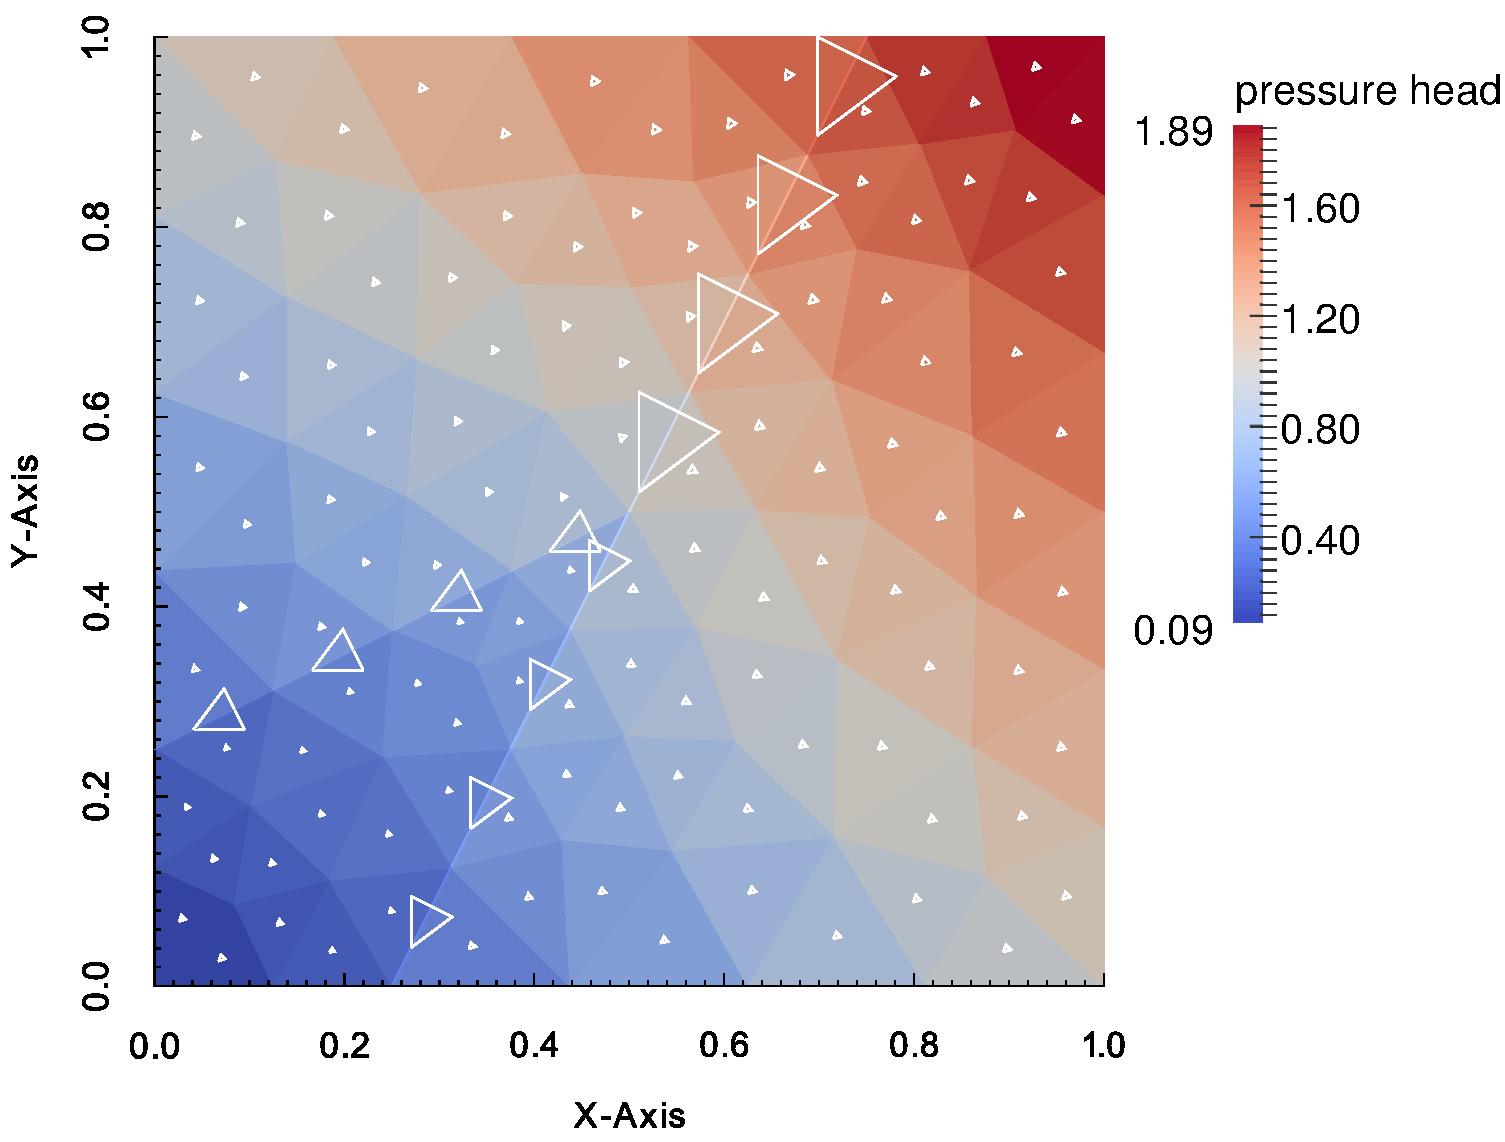
\includegraphics[width=\textwidth]{\fig/03_flow.pdf}
        % 03_flow.pdf: no raster
        \caption{Elementwise pressure head and\\velocity field denoted by triangles.\\ (Steady flow.)}
        \label{fig:tut-flow}
    \end{subfigure}
    ~
    \begin{subfigure}[b]{0.48\textwidth}
        \centering
        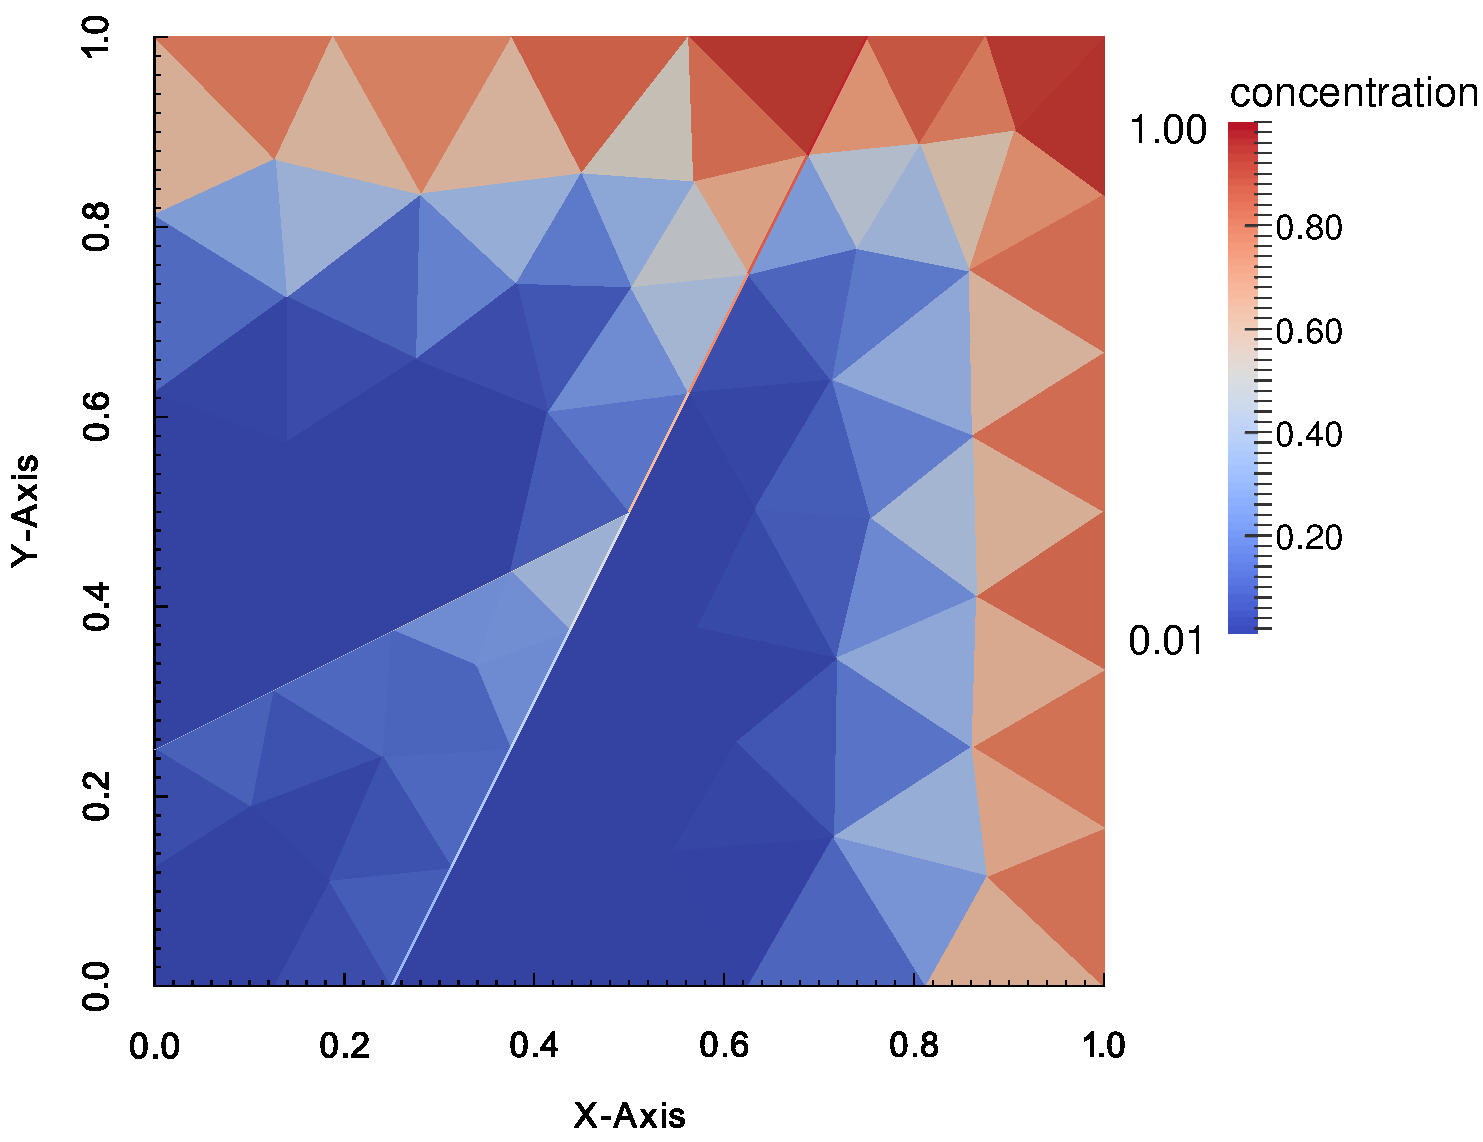
\includegraphics[width=\textwidth]{\fig/03_trans.pdf}
        % 03_trans.pdf: no raster
        \caption{Propagation of U235 from the inflow part of the boundary. \\ (At the time $9\cdot10^{5}$ s.)}
        \label{fig:tut-trans}
    \end{subfigure}
    \caption{Results of the tutorial problem.}
    \label{fig:tutorial}
\end{figure}


% In the following chapter we describe mathematical models used in Flow123d.
% Then in chapter \ref{chapter:file-formats} we briefly describe structure of individual input files, in particular the main CON file.
% The complete description of the CON format is given in chapter \ref{chapter:input-tree-reference}.


% \chapter[Mathematical Models of Physical Reality]{Mathematical Models \\of Physical Reality}
% \label{chapter:mathematical_models}

% Flow123d provides models for Darcy flow in porous media as well as for the transport and reactions of solutes. In this section, we describe 
% mathematical formulations of these models together with physical meaning and units of all involved quantities. In the first section we present 
% basic notation and assumptions about computational domains and meshes that combine different dimensions. In the next section we
% derive approximation of thin fractures by lower dimensional interfaces for a general transport process. Latter sections describe details for models of particular
% physical processes.

% \section{Meshes of Mixed Dimension}
% Unique feature common to all models in Flow123d is the support of
% domains with mixed dimension. 
% Let $\Omega_{3} \subset \Real^3$ be an open set representing continuous approximation of porous and fractured medium.
% Similarly, we consider a set of 2D manifolds $\Omega_2\subset\overline\Omega_3$, representing the 2D fractures and a set of 1D manifolds $\Omega_1\subset \overline\Omega_2$ 
% representing the 1D channels or preferential paths (see Fig \ref{fig:multi-dim}).
% We assume that $\Omega_2$ and $\Omega_1$ are polytopic (i.e. polygonal and piecewise linear, respectively).
% For every dimension $d=1,2,3$, we introduce a triangulation $\mathcal{T}_{d}$ of the open set $\Omega_d$
% that consists of finite elements $T_{d}^{i},$\ $i = 1,\dots,N_{E}^{d}$.
% The elements are simplices, i.e. lines, triangles and tetrahedra, respectively.

% \begin{figure}[h]
% \centering
% 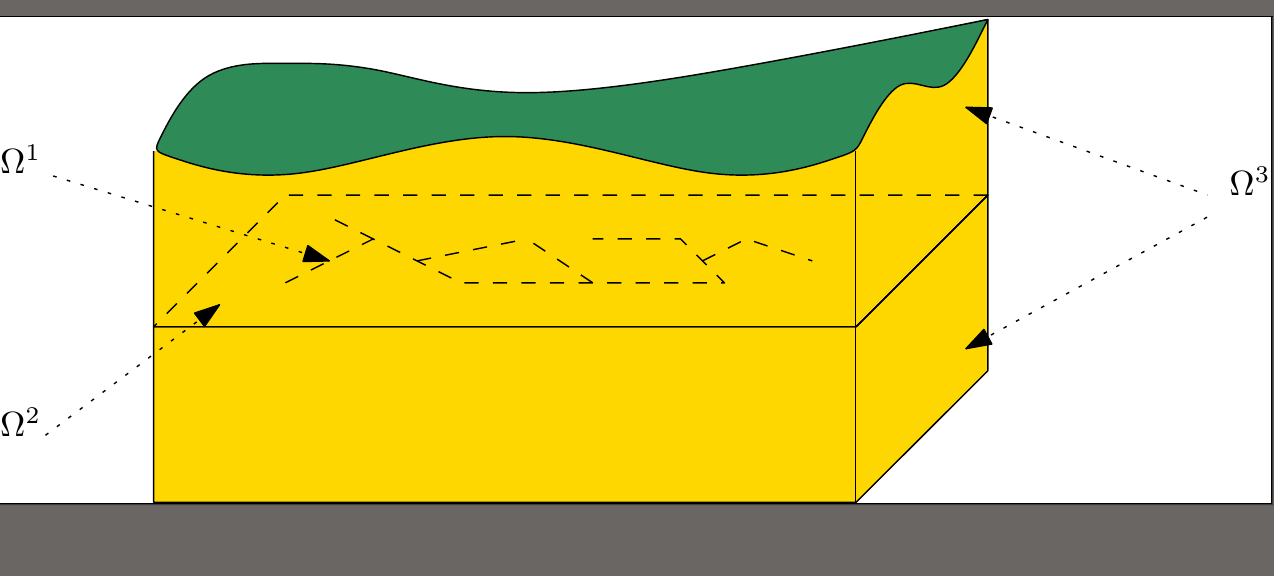
\includegraphics[width=10cm]{\fig/ground_fractures}
% \caption{
%     \label{fig:multi-dim}
%     Scheme of a problem with domains of multiple dimensions.
% }
% \end{figure}

% Present numerical methods used by the software require meshes satisfying the compatibility conditions
% \begin{equation}
%         T_{d-1}^i \cap T_d \subset \mathcal{F}_d,   \qquad \text{where } \mathcal{F}_d = \bigcup_{k} \partial T_{d}^{k}
% \end{equation}
% and
% \begin{equation}
%         T_{d-1}^i \cap \mathcal{F}_d    \text{ is either $T_{d-1}^i$ or $\emptyset$}    
% \end{equation}
% for every $i\in\{1,\dots, N_{E}^{d-1}\}$, $j\in\{1,\dots,N_{E}^{d}\}$,  and $d=2,3$. 
% That is, the $(d-1)$-dimensional elements are either between $d$-dimensional elements and
% match their sides or they poke out of $\Omega_d$. Support for a coupling between non-compatible
% meshes of different dimesion is in developement and partly supported by the Darcy Flow model.

% \section{Advection-Diffusion Processes on Fractures}
% \label{sc:ad_on_fractures}
% This section presents derivation of an abstract advection-diffusion process on 2D and 1D manifolds and its coupling with
% the higher dimensional domains. The reader not interested in the details of this approximation may skip directly to
% the later sections describing mathematical models of individual physical processes.

% As was already mentioned, the unique feature of Flow123d is support of models living on 2D and 1D manifolds. The aim is to capture 
% features significantly influencing the solution despite of their small cross-section. Such a tiny features are
% challenging for numerical simulations since a direct discretization requires highly refined
% computational mesh. One possible solution is to model these features (fractures, channels) 
% as lower dimensional objects (2D and 1D manifolds) and introduce their coupling with the surrounding continuum.
% The equations modeling a physical process on a manifold as well as its coupling to the model in the surrounding continuum
% has to be derived from the model on the 3D continuum. This section presents such a procedure for the case of the abstract
% advection-diffusion process inspired by the paper \cite{martin_modeling_2005}. Later, we this abstract approach to 
% particular advection-diffusion processes: Darcian flow, solute transport, and heat transfer.

% Let us consider a fracture as a strip domain 
% \[
%  \Omega_f \subset [0,\delta] \times \Real^{d-1}
% \]
% for $d=2$ or $d=3$ and surrounding continuum domains
% \[
%  \Omega_1 \subset (-\infty,0)\times \Real^{d-1},
%  \Omega_2 \subset (\delta,\infty)\times \Real^{d-1}.
% \]
% Further, we denote by $\gamma_i$, $i=1,2$ the fracture faces common with domains $\Omega_1$ and $\Omega_2$ respectively.
% By $x$, $\vc y$ we denote normal and tangential coordinate of a point in $\Omega_f$. 
% We consider the normal vector  $\vc n=\vc n_1=-\vc n_2=(1,0,0)^\top$.
% An advection-diffusion process is given by equations:
% \begin{align}
%   \label{eq:fr:continuity}
%   \prtl_t w_i + \div \vc j_i &= f_i&&  \text{on } \Omega_i,\ i=1,2,f,\\
%   \label{eq:fr:flux}
%   \vc j_i &= - \tn A_i\grad u_i + \vc b_i w_i&& \text{on } \Omega_i,\ i=1,2,f,\\
%   \label{eq:fr:Dirichlet}
%   u_i &= u_f&& \text{on } \gamma_i,\ i=1,2,\\
%   \label{eq:fr:Neumann}
%   \vc j_i \cdot \vc n &= \vc j_f \cdot \vc n&& \text{on } \gamma_i,\ i=1,2,
% \end{align}
% where $w_i=w_i(u_i)$ is the conservative quantity and $u_i$ is the principal unknown, $\vc j_i$ is the flux of $w_i$, $f_i$ is the source term,
% $\tn A_i$ is the diffusivity tensor and $\vc b_i$ is the velocity field. We assume that the tensor $\tn A_f$ is symmetric positive definite 
% with one eigenvector in the direction $\vc n$. Consequently the tensor has the form:
% \[
%  A_f = \begin{pmatrix} 
%             a_n & 0  \\
%             0 & \tn A_t
%        \end{pmatrix}
% \]
% Furthermore, we assume that $\tn A_f(x, \vc y)=\tn A_f(\vc y)$ is constant in the normal direction.

% Our next aim is to integrate equations on the fracture $\Omega_f$ in the normal direction 
% and obtain their approximations on the surface $\gamma=\Omega_f \cap \{x=\delta/2\}$ running through the middle of the fracture. 
% For the sake of clarity, we will not write subscript $f$ for quantities on the fracture. 
% To make the following procedure mathematicaly correct we have to assume that functions
% $\prtl_x w$, $\prtl_x \grad_{\vc y} u$, $\prtl_x \vc b_{\vc y}$ are continuous and bounded on $\Omega_f$. Here and later on 
% $\vc b_x=(\vc b \cdot \vc n)\, \vc n$ is the normal part of the velocity field and $\vc b_{\vc y} = \vc b - \vc b_x$ is the tangential part.
% The same notation will be used for normal and tangential part of the field $\vc q$.

% We integrate \eqref{eq:fr:continuity} over the fracture opening $[0,\delta]$ and use approximations to get
% \begin{equation}
%     \label{eq:fracture_continuity}
%    \prtl_t (\delta W) - \vc j_2 \cdot \vc n_2 - \vc j_1 \cdot \vc n_1 + \div \vc J = \delta F,
% \end{equation}
% where for the first term, we have used mean value theorem, first order Taylor expansion, 
% and boundedness of $\prtl_x w$ to obtain approximation:
% \[
%     \int_0^\delta w(x,\vc y) \d x=\delta w(\xi_{\vc y}, \vc y) = \delta W(\vc y) + O(\delta^2\abs{\prtl_x w}),
% \]
% where
% \[
%     W(\vc y)=w(\delta / 2,\vc y)=w(u(\delta/2,\vc y))=w(U(\vc y)).
% \]
% Next two terms in \eqref{eq:fracture_continuity} come from the exact integration 
% of the divergence of the normal flux $\vc j_x$.
% Integration of the divergence of the tangential flux $\vc j_{\vc y}$ gives the fourth term, where we introduced
% \[
% \vc J(\vc y) = \int_0^\delta \vc j_{\vc y}(x, \vc y) \d x.
% \]
% In fact, this flux on $\gamma$ is scalar for the case $d=2$. Finally, we integrate the right-hand side to get 
% \[
%     \int_0^\delta f(x,\vc y) \d x = \delta F(\vc y) + O(\delta^2\abs{\prtl_x f}),\quad F(\vc y)=f(\delta/2,\vc y). 
% \]


% Due to the particular form of the tensor $\tn A_f$, we can separately integrate tangential and normal
% part of the flux given by \eqref{eq:fr:flux}. Integrating the tangential part and using approximations
% \[
%     \int_0^\delta  \grad_{\vc y} u(x, \vc y) \d x = \delta \grad_{\vc y} u (\xi_{\vc y}, \vc y) 
%     = \delta \grad_{\vc y} U( \vc y) + O\big( \delta^2 \abs{\prtl_x\grad_{\vc y} u} \big) 
% \]
% and
% \[
%  \int_0^\delta \big(\vc b_{\vc y} w\big)(x, \vc y) \d x 
%   = \delta \vc B(\vc y) W(\vc y) + O\big(\delta^2 \abs{\prtl_x(\vc b_{\vc y} w)} \big)
% \]
% where
% \[
%   \vc B(\vc y) = \vc b_{\vc y}(\delta/2, \vc y),
% \]
% we obtain
% \begin{equation}
%     \label{eq:fracture_darcy}
%    \vc J = -\tn A_t \delta \grad_{\vc y} U + \delta \vc B W + O\big(\delta^2(\abs{\prtl_x\grad_{\vc y} u}+\abs{\prtl_x(\vc b_{\vc y} w)})\big).
% \end{equation}


% So far, we have derived equations for the state quantities $U$ and $\vc J$ on the fracture manifold $\gamma$. In order to
% get a well possed problem, we have to prescribe two conditions for boundaries $\gamma_i$, $i=1,2$. To this end, we
% perform integration of the normal flux $\vc j_x$, given by \eqref{eq:fr:flux}, separately for the left and right half of the fracture.
% Similarly as before we use approximations
% \[
%  \int_0^{\delta/2} \vc j_x \d x = (\vc j_1 \cdot \vc n_1)\frac{\delta}{2} + O(\delta^2 \abs{\prtl_x \vc j_x})
% \]
% and 
% \[
%  \int_0^{\delta/2} \vc b_x w \d x = (\vc b_1 \cdot \vc n_1)\tilde{w}_1\frac{\delta}{2} + O(\delta^2 \abs{\prtl_x \vc b_x}\abs{w} + \delta^2\abs{\vc b_x}\abs{\prtl_x w})
% \]
% and their counter parts on the interval $(\delta/2, \delta)$ to get
% \begin{align}
%     \label{eq:fracture_normal_1}
%      \vc j_1 \cdot \vc n_1 &= -\frac{2a_n}{\delta} (U - u_1) + \vc b_1\cdot \vc n_1 \tilde{w}_1\\
%     \label{eq:fracture_normal_2}
%     \vc j_2 \cdot \vc n_2 &= -\frac{2a_n}{\delta} (U - u_2) + \vc b_2\cdot \vc n_2 \tilde{w}_2
% \end{align}
% where $\tilde w_i$ can be any convex combination of $w_i$ and $W$. Equations \eqref{eq:fracture_normal_1}  
% and \eqref{eq:fracture_normal_2} have meaning of a semi-discretized flux from domains $\Omega_i$ into fracture.
% In order to get a stable numerical scheme, we introduce a kind of upwind already on this level using a different convex 
% combination for each flow direction:
% \begin{align}
%    \notag 
%    \vc j_i \cdot \vc n_i
%        = &-\sigma_i (U - u_i)      \\ 
%    \notag
%       &+ \big[\vc b_i\cdot \vc n_i\big]^{+} \big(\xi w_i + (1-\xi) W\big)       \\
%       \label{eq:fracture_normal}
%       &+ \big[\vc b_i\cdot \vc n_i\big]^{-} \big((1-\xi) w_i + \xi W\big), \qquad i=1,2
% \end{align}
% where $\sigma_i = \frac{2a_n}{\delta}$ is the transition coefficient and the parameter $\xi\in [\frac12, 1]$ can be used to interpolate
% between upwind ($\xi = 1$) and central difference ($\xi=\frac12$) scheme. Equations \eqref{eq:fracture_continuity}, \eqref{eq:fracture_darcy}, and
% \eqref{eq:fracture_normal} describe the general form of the advection-diffusion process on the fracture and its communication with 
% the surrounding continuum which we shall later apply to individual processes.


% 
\section{Darcy Flow Model} \label{sec:darcy_flow}
We consider the simplest model for the velocity of the steady or unsteady flow in porous and fractured medium given by 
the Darcy flow:
\begin{equation}
    \label{eq:darcy}
    \vc w = -\tn K \grad H \quad\text{in }\Omega_d,\ \text{for $d=1,2,3$}.
\end{equation}
Here and later on, we drop the dimension index $d$ of the quantities if it can be deduced from the context.
In \eqref{eq:darcy}, $\vc w$ \units{}{1}{-1} is \href{http://en.wikipedia.org/wiki/Superficial_velocity}{the superficial velocity},
$\tn K_d$ is the conductivity tensor, and $H$ \units{}{1}{} is the piezometric head. The velocity $\vc w_d$ is related to the flux $\vc q_d$ 
\units{}{4-d}{-1} through
\[
    \vc q_d = \delta_d \vc w_d,
\]
where $\delta_d$ \units{}{3-d}{} is the \hyperA{DarcyFlowMH-Data::cross-section}{cross section} coefficient,
in particular $\delta_3=1$, $\delta_2$ \units{}{1}{} is the thickness of a fracture, and $\delta_1$ \units{}{2}{} is the cross-section of a channel.
The flux $\vc q_d\cdot\vc n$ is the volume of the liquid (water) that passes through a unit square ($d=3$),
unit line ($d=2$), or through a point ($d=1$) per one second. 
The conductivity tensor is given by the product \penalty-500
$\tn K_d = k_d \tn A_d$, where $k_d>0$ \units{}{1}{-1}
 is the \hyperA{DarcyFlowMH-Data::conductivity}{hydraulic conductivity}  and 
$\tn A_d$  is the 
$3\times 3$ dimensionless \hyperA{DarcyFlowMH-Data::anisotropy}{anisotropy tensor} which has to be symmetric and positive definite.
The piezometric-head $H_d$ is related to the pressure head
$h_d$ through
\begin{equation}
    \label{eq:piezo_head}
    H_d = h_d + z
\end{equation}
assuming that the gravity force acts in the negative direction of the $z$-axis. 
Combining these relations, we get the Darcy law in the form:
\begin{equation}
    \label{eq:darcy_flux}
    \vc q = -\delta k\tn A \grad (h+z)  \qquad\text{in }\Omega_d,\ \text{for $d=1,2,3$}.
\end{equation}

Next, we employ the continuity equation for saturated porous medium and the dimensional reduction from the preceding section
(with $w=u:=H$, $\vc j:=\vc w$, $\tn A:=\tn K$ and $\vc b:=\vc 0$), which yields:
\begin{equation}
    \label{eq:continuity}
    \prtl_t (\delta S\, h) + \div \vc q = F \qquad \text{in }\Omega_d,\ \text{for $d=1,2,3$},
\end{equation}
where  $S_d$ \units{}{-1}{} is the \hyperA{DarcyFlowMH-Data::storativity}{storativity} and $F_d$ \units{}{3-d}{-1} is 
the source term. In our setting the principal unknowns of the system 
(\ref{eq:darcy_flux}, \ref{eq:continuity}) are the pressure head $h_d$ and the flux $\vc q_d$.


The storativity (or the volumetric specific storage) $S_d>0$ can be expressed as
\begin{equation}
  S_d = \gamma_w(\beta_r + \vartheta \beta_w),
\end{equation}
where $\gamma_w$ \units{1}{-2}{-2} is the specific weight of water, $\vartheta$ \units{}{}{} is the porosity,
$\beta_r$ is compressibility of the bulk material of the pores (rock)
and $\beta_w$ is compressibility of the water, both with units \units{-1}{1}{-2}. For steady problems, we set $S_d=0$ for all dimensions $d=1,2,3$.
The source term $F_d$ on the right hand side of \eqref{eq:continuity} consists of the volume density of the 
\hyperA{DarcyFlowMH-Data::water-source-density}{water source} 
 $f_d$\units{}{}{-1} and flux from the from the higher dimension. 
Precise form of $F_d$ slightly differs for every dimension and will be discussed presently.

In $\Omega_3$ we simply have $F_3  = f_3$ \units{}{}{-1}.

In the set $\Omega_2 \cap \Omega_3$ the fracture is surrounded by at most one 3D surface from every side.
On $\prtl\Omega_3 \cap \Omega_2$ we prescribe a boundary condition of the Robin type:
\begin{align*}
        \vc{q}_3\cdot \vc n^{+} &= q_{32}^{+} =\sigma_{3} (h_3^{+}-h_2),\\
        \vc{q}_3\cdot \vc n^{-} &= q_{32}^{-} =\sigma_{3} (h_3^{-}-h_2),
\end{align*}
where $\vc{q}_3\cdot\vc n^{+/-}$ \units{}{1}{-1} is the outflow from $\Omega_3$, $h_3^{+/-}$ is
a trace of the pressure head in $\Omega_3$, $h_2$ is the pressure head in $\Omega_2$, and 
$\sigma_{3}$ \units{}{}{-1} is the transition coefficient given by (see section \ref{sc:ad_on_fractures} and \cite{martin_modeling_2005})
\[
\label{e:sigma3_law}
  \sigma_3 = \sigma_{32} \frac{2\tn K_2 :\vc n_2\otimes\vc n_2 }{\delta_2}.
\]
Here $\vc n_2$ is the unit normal to the fracture (sign does not matter).
On the other hand, the sum of the interchange fluxes $q_{32}^{+/-}$ forms
a volume source in $\Omega_2$.  Therefore $F_2$ \units{}{1}{-1} on the right hand side of \eqref{eq:continuity} is
given by
\begin{equation}
   \label{source_2D}
   F_2 = \delta_2 f_2 + (q_{32}^{+} + q_{32}^{-}).
\end{equation}

The communication between $\Omega_2$  and  $\Omega_1$ is similar.  However, in the 3D ambient space,
a 1D channel can join multiple 2D fractures $1,\dots, n$. Therefore, we have $n$
independent outflows from $\Omega_2$:
\begin{equation*}
        \vc{q}_2\cdot \vc n^{i} = q_{21}^{i} =\sigma_{2} (h_2^{i}-h_1),
\end{equation*}
where $\sigma_2$ \units{}{1}{-1} is the transition coefficient integrated over the width of the fracture $i$:
\[
\label{e:sigma2_law}
  \sigma_2 = \sigma_{21} \frac{2\delta_2^2\tn K_1:{\vc n_1^i}\otimes{\vc n_1^i}}{\delta_1}.
\]
Here $\vc n_1^i$ is the unit normal to the channel that is tangential to the fracture $i$.
Sum of the fluxes forms a part of $F_1$ \units{}{2}{-1}:
\begin{equation}
   \label{source_1D}
   F_1 = \delta_1 f_1 + \sum_{i=1}^n q_{21}^{i}. 
\end{equation}
We remark that the direct communication between 3D and 1D (e.g. model of a well) is not supported yet.
The \hyperA{DarcyFlowMH-Data::sigma}{transition coefficients} 
{$\sigma_{32}$} \units{}{}{} and
{$\sigma_{21}$} \units{}{}{} are independent scaling parameters which represent 
the ratio of the crosswind and the tangential conductivity in the fracture. For example, in the case of impermeable film
on the fracture walls one may choice $\sigma_{32} < 1$.

In order to obtain unique solution we have to prescribe boundary conditions. Currently we support three basic 
\hyperA{DarcyFlowMH-Data::bc-type}{types of boundary conditions}:

{\bf Dirichlet} boundary condition
\[
    h_d = h_d^D        \text{ on }\Gamma_d^D,
\]
where $h_d^D$ \units{}{1}{} is the \hyperA{DarcyFlowMH-Data::bc-pressure}{boundary pressure head} .
Alternatively one can prescribe the \hyperA{DarcyFlowMH-Data::bc-piezo-head}{boundary piezometric head}
$H_d^D$ \units{}{1}{} related to the pressure head through \eqref{eq:piezo_head}.

{\bf Neuman} boundary condition
\[
    \vc q_d \cdot \vc n = q_d^N         \text{ on }\Gamma_d^N,
\]
where $q_d^N$ \units{}{4-d}{-1} is the \hyperA{DarcyFlowMH-Data::bc-flux}{surface density of the water outflow}.

{\bf Robin} boundary condition 
\[
    \vc q_d \cdot \vc n = \sigma_d^R ( h_d - h_d^R)     \text{ on }\Gamma_d^R.
\]
where $h_d^R$ is the \Alink{DarcyFlowMH-Data::bc-pressure}{boundary pressure head} and
$\sigma_d^R$ \units{}{3-d}{-1} {} 
is the \hyperA{DarcyFlowMH-Data::bc-robin-sigma}{transition coefficient}.
As before one can also prescribe the \Alink{DarcyFlowMH-Data::bc-piezo-head}{boundary piezo head}
$H_d^R$ to specify $h_d^R$.

We consider a disjoint decomposition of the boundary
\[
    \prtl\Omega_d =  \cap \Gamma_d^N \cap \Gamma_d^R
\]
into Dirichlet, Neumann, and Robin part. In order to obtain well posed steady state problem one have to 
prescribe Dirichlet or Robin boundary condition on part of boundary that is connected (geometricaly of through
the inter dimensional coupling) to hte rest of the domain.

For unsteady problems one has to specify an initial condition in terms of the 
\hyperA{DarcyFlowMH-Data::init-pressure}{initial pressure head}
$h_d^0$ \units{}{1}{}
or the \hyperA{DarcyFlowMH-Data::init-piezo-head}{initial piezometric head}
$H_d^0$ \units{}{1}{}.

\paragraph{Volume balance.}
The equation \eqref{eq:continuity} satisfies the volume balance of the liquid in the following form:
\[ V(0) + \int_0^t s(\tau) \,d\tau - \int_0^t f(\tau) \,d\tau = V(t) \]
for any instant $t$ in the computational time interval.
Here
$$ V(t) := \sum_{d=1}^3\int_{\Omega^d}(\delta S h)(t,\vc x)\,d\vc x, $$
$$ s(t) := \sum_{d=1}^3\int_{\Omega^d}F(t,\vc x)\,d\vc x, $$
$$ f(t) := \sum_{d=1}^3\int_{\partial\Omega^d}\vc q(t,\vc x)\cdot\vc n(\vc x) \,d\vc x $$
is the volume \units{}{3}{}, the volume source \units{}{3}{-1} and the volume flux \units{}{3}{-1} of the liquid at time $t$, respectively.
The volume, flux and source on every geometrical region is calculated at each computational time step and the values together with the control sums are written to the file \texttt{water\_balance.txt}.






% % ***************************************** SYMBOLS
\def\abs#1{\lvert#1\rvert}
\def\argdot{{\hspace{0.18em}\cdot\hspace{0.18em}}}
% \def\avg#1{\left\{#1\right\}_\omega}
\def\D{{\tn D}}
\def\div{\operatorname{div}}
% \def\Eh{\mathcal E_h}       % edges of \Th
% \def\Ehcom{\mathcal E_{h,C}}         % edges of \Th on interface with lower dimension
% \def\Ehdir{\mathcal E_{h,D}}         % Dirichlet edges of \Th
% \def\Ehint{\mathcal E_{h,I}}       % interior edges of \Th
\def\grad{\nabla}
% \def\jmp#1{[#1]}
\def\n{\vc n}
\def\vc#1{\mathbf{\boldsymbol{#1}}}     % vector
\def\R{\mathbb R}
\def\sc#1#2{\left(#1,#2\right)}
% \def\Th{\mathcal T_h}       % triangulation
\def\th{\vartheta}
% \def\tn#1{{\mathbb{#1}}}    % tensor
\def\Tr{\operatorname{Tr}}
\def\where{\,|\,}
%***************************************************************************


\section{Transport of Substances}
\label{sc:transport_model}

The motion of substances dissolved in water is governed by the \emph{advection}, and the \emph{hydrodynamic dispersion}.
In $\Omega_d$, $d\in\{1,2,3\}$, we consider the following system of mass balance equations\footnote{For $d\in\{1,2\}$ this form can be derived as in Section \ref{sc:ad_on_fractures} using $w:=\delta\th c^i$, $u:=c^i$, $\tn A:=\delta\th\tn D^i$, $\vc b:=\vc v=\frac{\vc q}{\th\delta}$.}:
\begin{equation}
    \label{e:ADE}
   \partial_t ( \delta \th c^i) + \div ( \vc q c^i ) - \div (\th \delta \D^i \grad c^i ) = F_S^i + F^c_C + F_R(c^1,\dots, c^s).
\end{equation}
The principal unknown is the concentration $c^i$ \units{1}{-3}{} of a substance $i\in\{1,\dots, s\}$, which means the weight of the substance in the unit volume of water.
Other quantities are:
\begin{itemize}
\item The \hyperA{SoluteTransport-DG-Data::porosity}{porosity} $\th$ \units{}{}{}, i.e. the fraction of space occupied by water and the total volume.
\item The hydrodynamic dispersivity tensor $\D^i$ \units{}{2}{-1} has the form
\begin{equation} 
  \label{eqn:transport_disp}
  \D^i =D_m^i \tau \tn I + \abs{\vc v}\left(\alpha_T^i \tn I + (\alpha_L^i - \alpha_T^i) \frac{\vc v \otimes \vc v}{\abs{\vc v}^2}\right),
\end{equation}
which represents (isotropic) molecular diffusion, and mechanical dispersion in longitudal and transversal direction to the flow.
Here $D_m^i$ \units{}{2}{-1} is the \hyperA{SoluteTransport-DG-Data::diff-m}{molecular diffusion coefficient} of the $i$-th substance (usual magnitude in clear water is $10^{-9}$), $\tau=\th^{1/3}$ is the tortuosity (by \cite{millington_quirk}), $\alpha_L^i$ \units{}{1}{} and $\alpha_T^i$ \units{}{1}{} is the \hyperA{SoluteTransport-DG-Data::disp-l}{longitudal dispersivity} and the \hyperA{SoluteTransport-DG-Data::disp-t}{transverse dispersivity}, respectively.
Note that although we allow dispersivities to have different values for different substances, it is often assumed that they are intrinsic parameters of the porous medium.
Finally, $\vc v$ \units{}{1}{-1} is the \emph{microscopic} water velocity, related to the Darcy flux $\vc q$ by the relation $\vc q = \th\delta\vc v$.
The value of $D_m^i$ for specific substances can be found in literature (see e.g. \cite{cislerova_vogel}).
For instructions on how to determine $\alpha_L^i$, $\alpha_T^i$ we refer to \cite{marsily,domenico_schwartz}.

\item $F_S^i$ \units{1}{-d}{-1} represents the density of concentration sources in the porous medium.
Its form is:
\begin{equation}
 F_S^i = \delta f^i_S + \delta(c_S^i-c^i)\sigma_S^i. \label{eqn:transport_sources}
\end{equation}
Here $f_S^i$ \units{1}{-3}{-1} is the \hyperA{SoluteTransport-DG-Data::sources-density}{density of concentration sources}, $c_S^i$ \units{1}{-3}{} is an \hyperA{SoluteTransport-DG-Data::sources-conc}{equilibrium concentration} and $\sigma_S^i$ \units{}{}{-1} is the \hyperA{SoluteTransport-DG-Data::sources-sigma}{concentration flux}.
One has to pay attention when prescribing the source, namely to determine whether it is related to the \emph{liquid} or the \emph{porous medium}. We mention several examples:
\begin{itemize}
\item extraction of solution: $f_S^i = 0$, $c_S^i = 0$, $\sigma_S^i>0$ is the intensity of extraction, i.e. volume of liquid extracted from a unit volume of porous medium per second;
\item injection of solution: $f_S^i = 0$, $c_S^i$ is the concentration of the substance in the injected liquid, $\sigma_S^i>0$ is the intensity of injection (volume of liquid injected into a unit volume of porous medium per second);
% \item source of contamination
\item production or degradation of substances due to bacteria present in liquid: $f_S^i=\th p^i$, where $p^i$ is the production/degradation rate in a unit volume of liquid;
\item age of liquid: if $f_S^i=\th$ then $c^i$ is the age of liquid, i.e. the time spent in the domain.
\end{itemize}

\item $F^c_C$ \units{1}{-d}{-1} is the density of concentration sources due to exchange between regions with different dimensions, see \eqref{e:FC} below.

\item The reaction term $F_R(\dots)$ \units{1}{-d}{-1} is thoroughly described in the next section \ref{sec:reaction_term}.
\end{itemize}



\paragraph{Initial and boundary conditions.}
At time $t=0$ the concentration is determined by the \hyperA{SoluteTransport-DG-Data::init-conc}{initial condition}
$$ c^i(0,\vc x) = c^i_0(\vc x). $$
The physical boundary $\partial\Omega_d$ is decomposed into the parts $\Gamma_I\cup\Gamma_D\cup\Gamma_N\cup\Gamma_R$, which may change during simulation time.
The first part $\Gamma_I$ is further divided into two segments:
\begin{align*}
\Gamma_I^+(t) &= \{\vc x\in \partial\Omega_d\where \vc q(t,\vc x)\cdot\vc n(\vc x)<0\},\\
\Gamma_I^-(t) &= \{\vc x\in \partial\Omega_d\where \vc q(t,\vc x)\cdot\vc n(\vc x)\ge 0\},
\end{align*}
where $\vc n$ stands for the unit outward normal vector to $\partial\Omega_d$.
We prescribe the following \hyperA{SoluteTransport-DG-Data::bc-type}{boundary conditions}:
On $\Gamma_D$, the Dirichlet condition is imposed via \hyperA{SoluteTransport-DG-Data::bc-conc}{prescribed concentration} $c_D^i$:
$$ c^i = c^i_D \mbox{ on }\Gamma_D. $$
On the inflow $\Gamma_I^+$ the \hyperA{SoluteTransport-DG-Data::bc-conc}{reference concentration} $c_D^i$ is enforced through total flux:
$$ (\vc q c^i - \th\delta\D^i\nabla c^i)\cdot\vc n = \vc q\cdot\vc n c_D^i \mbox{ on }\Gamma_I^+, $$
on $\Gamma_I^-$ we impose homogeneous Neumann condition:
$$ -\th\delta\D^i\nabla c^i\cdot\vc n = 0 \mbox{ on }\Gamma_I^-, $$
on $\Gamma_N$ we impose Neumann condition with user-defined \hyperA{SoluteTransport-DG-Data::bc-flux}{concentration flux} $f^i_N$:
$$ -\th\delta\D^i\nabla c^i\cdot\vc n = f^i_N \mbox{ on }\Gamma_N, $$
and finally on $\Gamma_R$ we impose Robin condition through \hyperA{SoluteTransport-DG-Data::bc-robin-sigma}{transition parameter} $\sigma^i_R$ and \hyperA{SoluteTransport-DG-Data::bc-conc}{reference concentration} $c^i_D$:
$$ -\th\delta\D^i\nabla c^i\cdot\vc n = \sigma^i_R(c^i-c^i_D) \mbox{ on }\Gamma_R. $$






\paragraph{Communication between dimensions.}
Transport of substances is considered also on interfaces of physical domains with adjacent dimensions (i.e. 3D-2D and 2D-1D, but not 3D-1D).
Denoting $c_{d+1}$, $c_d$ the concentration of a given substance in $\Omega_{d+1}$ and $\Omega_d$, respectively, the comunication on the interface between $\Omega_{d+1}$ and $\Omega_d$ is described by the quantity
\begin{equation}
  \label{e:inter_dim_flux}
  q^c_{d+1,d} = \sigma^c_{d+1,d} \frac{\delta_{d+1}^2}{\delta_d}2\th_d\D_d:\n\otimes\n ( c_{d+1} - c_d) + \begin{cases}q^l_{d+1,d} c_{d+1} & \mbox{ if }q^l_{d+1,d}\ge 0,\\q^l_{d+1,d} \frac{\th_d}{\th_{d+1}} c_d & \mbox{ if }q^l_{d+1,d}<0,\end{cases}
\end{equation}
where
\begin{itemize}
\item $q^c_{d+1,d}$ \units{1}{-d}{-1} is the density of concentration flux from $\Omega_{d+1}$ to $\Omega_d$,
\item $\sigma^c_{d+1,d}$ \units{}{}{} is a \hyperA{SoluteTransport-DG-Data::fracture-sigma}{transition parameter}.
Its value determines the mass exchange between dimensions whenever the concentrations differ.
In general, it is recommended to leave the default value $\sigma^c=1$ or to set $\sigma^c=0$ (when exchange is due to water flux only).
\item $q^l_{d+1,d}$ \units{}{3-d}{-1} is the water flux from $\Omega_{d+1}$ to $\Omega_d$, i.e. $q^l_{d+1,d} = \vc q_{d+1}\cdot\n_{d+1}$.
\end{itemize}
The communication between dimensions is incorporated as the total flux boundary condition for the problem on $\Omega_{d+1}$:
\begin{equation}
\label{e:FC}
-\th\delta\D\nabla c\cdot\vc n + q^l c = q^c
\end{equation}
and a source term in $\Omega_d$:
\begin{equation}
F^c_{C3} = 0,\quad
F^c_{C2} = q^c_{32},\quad
F^c_{C1} = q^c_{21}.
\end{equation}



\paragraph{Mass balance.}
The advection-dispersion equation satisfies the balance of mass in the following form:
$$ m^i(0) + \int_0^t s^i(\tau) \,d\tau - \int_0^t f^i(\tau) \,d\tau = m^i(t) $$
for any instant $t$ in the computational time interval and any substance $i$.
Here
$$ m^i(t) := \sum_{d=1}^3\int_{\Omega^d}(\delta\th c^i)(t,\vc x)\,d\vc x, $$
$$ s^i(t) := \sum_{d=1}^3\int_{\Omega^d}F_S^i(t,\vc x)\,d\vc x, $$
$$ f^i(t) := \sum_{d=1}^3\int_{\partial\Omega^d}\left(\vc q c^i - \th\delta\D^i\nabla c^i\right)(t,\vc x)\cdot\vc n \,d\vc x $$
is the mass \units{1}{}{}, the volume source \units{1}{}{-1} and the mass flux \units{1}{}{-1} of $i$-th substance at time $t$, respectively.
The mass, flux and source on every geometrical region is calculated at each computational time step and the values together with the control sums are written to the file \texttt{mass\_balance.txt}.


\paragraph{Two transport models.}
Within the above presented model, Flow123d presents two possible approaches to solute transport.
\begin{itemize}
\item For modelling pure advection ($\tn D=0$) one can choose {\tt TransportOperatorSplitting} method, which represents an explicit in time finite volume solver. 
Only the inflow/outflow boundary condition is available and the source term has the form
\[ F_S^i = \delta f_S^i + \delta(c_S^i-c^i)^+\sigma_S^i. \]
The solution process for one time step is faster, but the maximal time step is restricted. The resulting concentration is piecewise constant on mesh elements. This solver supports reaction term (involving simple chemical reactions, dual porosity and sorption).
\item The full model including dispersion is solved by {\tt SoluteTransport\_DG}, an implicit in time discontinuous Galerkin solver. It has no restriction of the computational time step and the space approximation is piecewise polynomial, currently up to order 3. Reaction term is currently not implemented.
\end{itemize}





% % ***************************************** SYMBOLS
\def\abs#1{\lvert#1\rvert}
\def\argdot{{\hspace{0.18em}\cdot\hspace{0.18em}}}
\def\avg#1{\left\{#1\right\}_\omega}
\def\D{{\tn D}}
\def\div{\operatorname{div}}
\def\Eh{\mathcal E_h}       % edges of \Th
\def\Ehcom{\mathcal E_{h,C}}         % edges of \Th on interface with lower dimension
\def\Ehdir{\mathcal E_{h,D}}         % Dirichlet edges of \Th
\def\Ehint{\mathcal E_{h,I}}       % interior edges of \Th
\def\grad{\nabla}
\def\jmp#1{[#1]}
\def\n{\vc n}
\def\vc#1{\mathbf{\boldsymbol{#1}}}     % vector
\def\R{\mathbb R}
\def\sc#1#2{\left(#1,#2\right)}
\def\Th{\mathcal T_h}       % triangulation
\def\th{\vartheta}
\def\tn#1{{\mathbb{#1}}}    % tensor
\def\Tr{\operatorname{Tr}}
\def\where{\,|\,}
%***************************************************************************

\section{Reaction Term in Transport}
\label{sec:reaction_term}

The {\tt TransportOperatorSplitting} method supports the reaction term $F_R(c^1,\ldots,c^s)$ on the right hand side of the equation (\ref{e:ADE}).
It can represent several models of chemical or physical nature. 
Figure \ref{fig:reaction_term} shows all possible reactional models that we support in combination with the transport process. The Operator Splitting method enables 
us to deal with the convection part and reaction term side by side. The convected quantities do not influence each other in the convectional
process and are balanced over the elements. On the other hand the reaction term relates the convected quantities and can be computed 
separately on each element.

We move now to the description of the reaction models which can be seen again in Figure \ref{fig:reaction_term}. 
The convected quantity is considered to be the concentration of substances. 
Up to now we can have \emph{dual porosity}, \emph{sorption} (these two are more of a physical nature) and (chemical) \emph{reaction} models in the reaction term. 

\begin{figure}
  \centering
  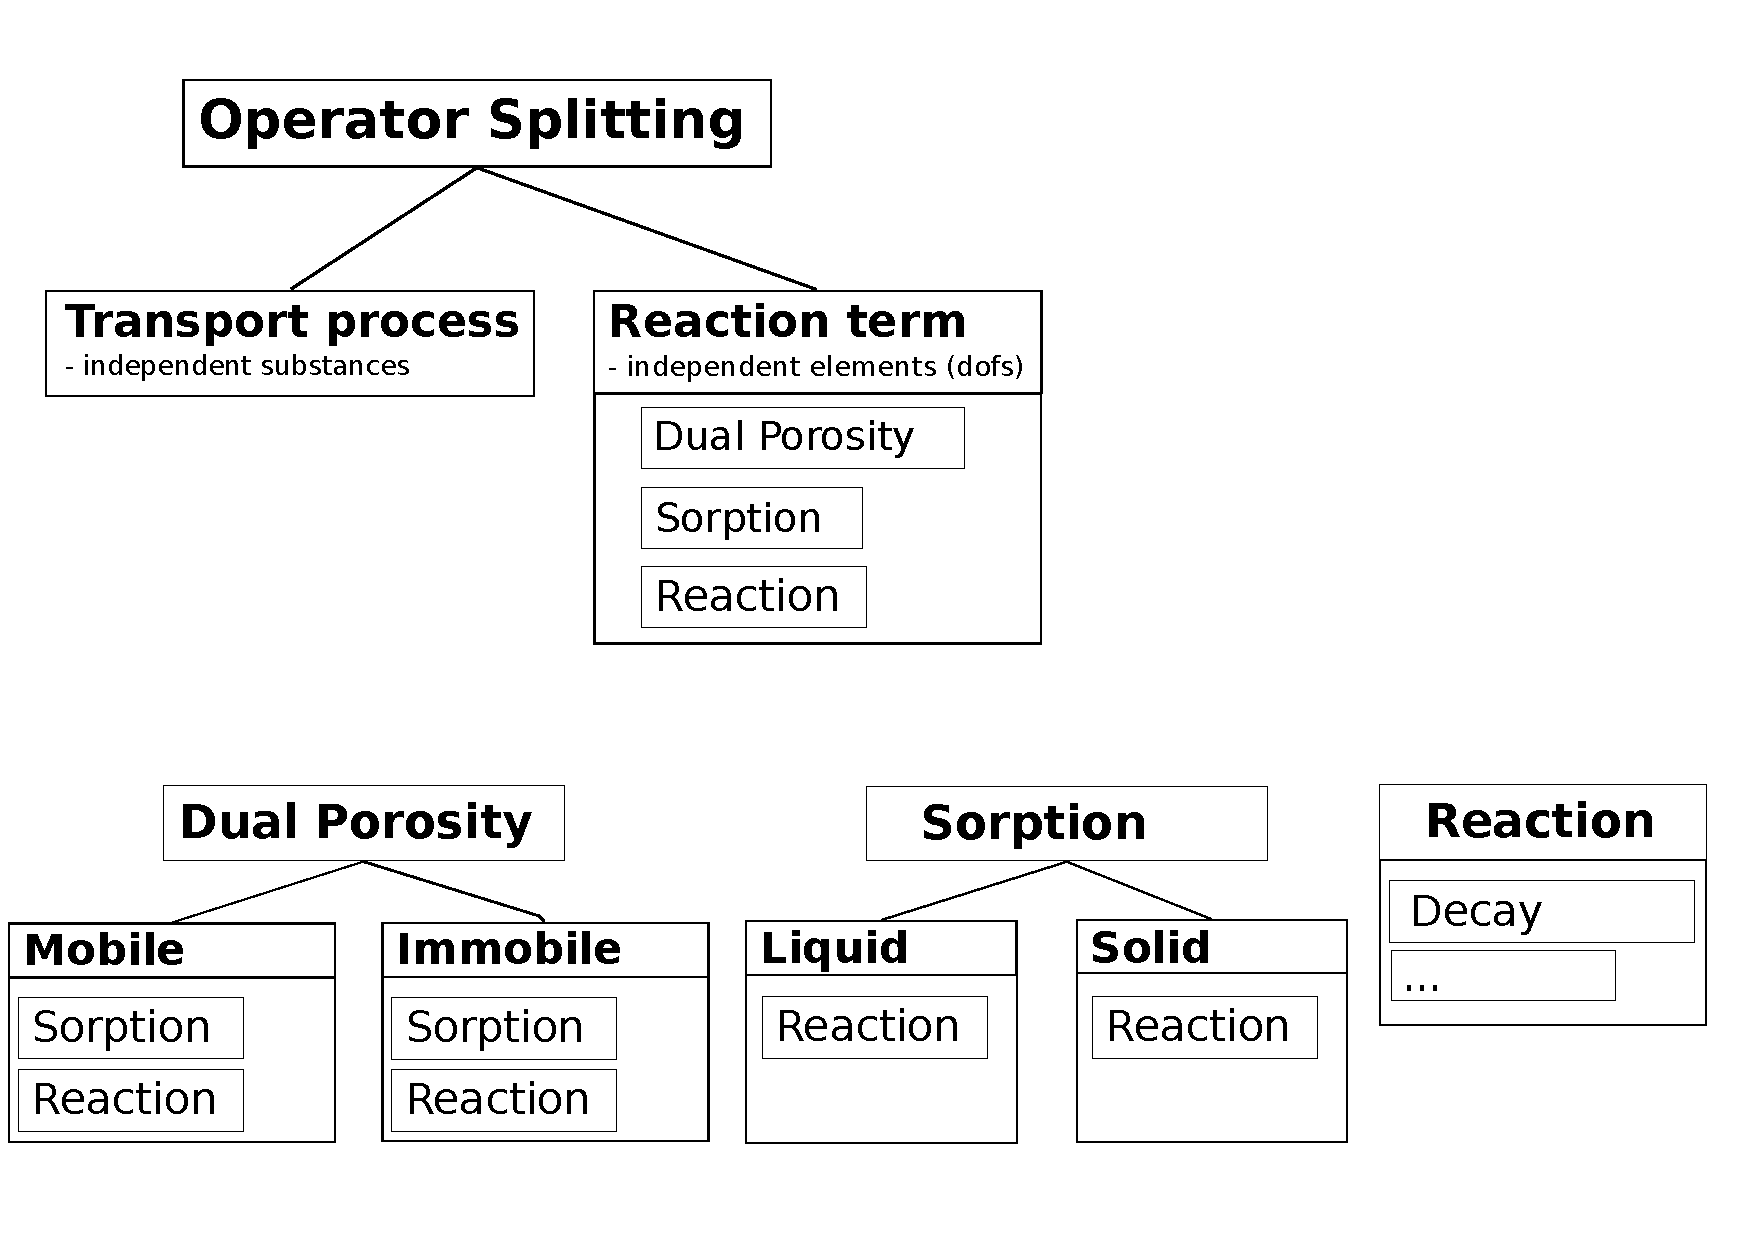
\includegraphics[width=\textwidth]{\fig/reaction_term.pdf}
  \caption{The scheme of the reaction term objects. The lines represents connections between different models. 
  The tables under model name include the possible models which can be connected to the model above.}
  \label{fig:reaction_term}
\end{figure}

The \emph{reaction} model acts only on the specified substances and computes exchange of concentration 
among them. It does not have its own output because it only changes the concentration of substances 
in the specified zone where the reaction takes place.
% See Section \ref{sec:linear_reactions} for thorough description.

The \emph{sorption} model describes the exchange of concentration of the substances between liquid and solid. It can be
followed by another \emph{reaction} that can run in both phases. The concentration in solid is an additional output 
of this model. See Subsection \ref{sec:sorp_math}.


The \emph{dual porosity} model, described in Subsection \ref{sec:dual_porosity}, introduces the so called immobile (or dead-end) pores in the matrix. 
The convection process operates only on the concentration of the substances in the mobile zone (open pores) 
and the exchange of concentrations from/to immobile zone is governed by molecular diffusion. This process can be followed by 
\emph{sorption} model and/or chemical \emph{reaction}, both in mobile and immobile zone. The immobile concentration is an
additional output.


\subsection{Dual Porosity} 
\label{sec:dual_porosity}

Up to now, we have described the transport equation for the single porosity model. The dual porosity model splits the mass into 
two zones -- the mobile zone and the immobile zone. Both occupy the same macroscopic volume, however on the microscopic scale, 
the immobile zone is formed by the dead-end pores, where the liquid is trapped and cannot pass through. The rest of the pore volume 
is occupied by the mobile zone. Since the liquid in the immobile pores is immobile, the exchange of the substance is only due 
to molecular diffusion. We consider simple nonequilibrium linear model:
\begin{subequations}
\label{eq:odes_dual_por}
\begin{align}
    \vartheta_m \partial_t c_m &= D_{dp} ( c_i - c_m), \label{eqn:dual_porosity_ode1}\\
    \vartheta_i \partial_t c_i &= D_{dp} ( c_m - c_i), \label{eqn:dual_porosity_ode2}
\end{align}
\end{subequations}
where $c_m$ is the concentration in the mobile zone, $c_i$ is the concentration in the immobile zone and
$D_{dp}$ is a \hyperA{DualPorosity-Data::diffusion-rate-immobile}{diffusion rate} between the zones.
$\vartheta_i$~denotes \hyperA{DualPorosity-Data::porosity-immobile}{porosity of the immobile zone} and 
$\vartheta_m = \vartheta$ the \hyperlink{TransportOperatorSplitting-Data::porosity::B}{mobile porosity} from 
transport equation \eqref{e:ADE}. One can also set non-zero \hyperA{DualPorosity-Data::init-conc-immobile}{initial 
concentration in the immobile zone} $c_i(0)$.

To solve the system of first order differential equation, we use analytic solution or Euler's method,
which are switched according to a given error tolerance. See subsection \ref{sec:num_dual_porosity} 
in numerical methods.
 

\subsection{Equilibrial Sorption}
\label{sec:sorp_math}

The simulation of monolayer, equilibrial sorption is based on the solution of two algebraic equations, namely the mass balance (in unit volume)
\begin{equation}
\label{eq:mass_balance_sorption}
\th \varrho_l c_l + (1-\th) \varrho_s M_s c_s = c_T = const.
\end{equation}
and an empirical sorption law
\begin{equation}
\label{eq:relation_cs_cl}
c_s = f(c_l),
\end{equation}
given in terms of the so-called isotherm $f$.
Its form is determined by the parameter \hyperA{Sorption-Data::sorption-type}{sorption type}:
\begin{itemize}
 \item ``$none$'': $f(c_l)=0$ (the sorption model returns zero concentration in solid);
 \item ``$linear$'': $f(c_l) = k_l c_l$;
 \item ``$freundlich$'': $f(c_l) = k_F c_l^{\alpha}$;
 \item ``$langmuir$'': $f(c_l) = k_L \frac{\alpha c_l}{1 + \alpha c_l}$.
       Langmuir isotherm has been derived from thermodynamic laws. $k_L$ denotes the maximal amount 
       of sorbing specie which can be kept in an unit volume of a bulk matrix. Coefficient $\alpha$ is 
       a fraction of sorption and desorption rate constant $\alpha = \frac{k_a}{k_d}$.
\end{itemize}

Notation:
\begin{itemize}
 \item In solid, $c_s = \frac{n}{m_s}$ [mol\,$\mathrm{kg}^{-1}$] is the fraction of the molar amount of the solute 
       adsorbed $n$ and the amount of the adsorbent $m_s$ (mass of solid), all in unit volume. The concentration
       in solid can be selected for \hyperA{Sorption::output-fields}{output}.
 \item In liquid, $c_l = \frac{m}{m_l}$ \units{}{}{} is the fraction of the amount of the solute $m$ and 
       the mass of liquid $m_l$, all in unit volume. The relation between $c_l$ and the concentration $c$ from 
       transport equation \eqref{e:ADE} is $c = c_l \varrho_l$.
 \item $\varrho_l$, $\varrho_s$ is the \hyperA{Sorption::solvent-density}{liquid (solvent) density} and 
       the \hyperA{Sorption-Data::rock-density}{solid (rock) density}, respectively.
 \item $M_s$ denotes the \hyperA{Substance::molar-mass}{molar mass} of a substance.
 \item \hyperA{Sorption-Data::isotherm-mult}{Multiplication parameters} are $k_i, i\in\{ l,F,L\}$ [mol\,$\mathrm{kg}^{-1}$].
 \item \hyperA{Sorption-Data::isotherm-other}{Additional parameter} $[\alpha] = 1$ can be set.
\end{itemize}

Non-zero \hyperA{Sorption-Data::init-conc-solid}{initial concentration} in the solid phase $c_s(0)$ can be set in the input record. 
Now, further denoting \[ \mu_l = \varrho_l \th, \quad \mu_s = M_s \varrho_s\cdot(1-\th), \]
and using \eqref{eq:relation_cs_cl}, the mass balance \eqref{eq:mass_balance_sorption} reduces to the equation
\begin{equation}
 c_T = \mu_l c_l + \mu_s f(c_l),
 \label{eq:nonlin_sorption}
\end{equation}
which can be either solved iteratively or using interpolation. See subsection \ref{sec:num_sorp_math} 
in numerical methods for details.

The units of $c_l$, $c_s$ and $k_i$ can vary in literature. To avoid misinterpretation, we derive (according
to Bowman~\cite{bowman_conversion_1982}) a conversion rule for Freundlich isotherm which will lead the user 
also in other cases, we believe. 

\paragraph{Units conversion.} Let us have $c$ \units{1}{-3}{}, the mass concentration in liquid, and $s$~[kg\,$\mathrm{kg}^{-1}$], 
the fraction of the amount of the solute adsorbed and the amount of the adsorbent in solid. 
The unit of $K$ follows from the dimensional analysis of $s=Kc^{\alpha}$:
\[[K] = \frac{\rm{kg}^{1-\alpha}\rm{m}^{3\alpha}}{\rm{kg}},\]
which we want to convert to $k_F$ [mol\,$\mathrm{kg}^{-1}$] in the formula $c_s=k_Fc_l^\alpha$.

The first step is a conversion of the mass of the solute to moles by dividing it by the
molar mass $M_s$. We then have the formula 
\begin{eqnarray}
s&=&Kc^{\alpha} \nonumber \\
\frac{s}{M_s} &=& K'\left(\frac{c}{M_s}\right)^\alpha, \label{eqn:sorp_molar_conc}\\
s &=& K'M_s^{1-\alpha}c^\alpha, \nonumber 
\end{eqnarray}
where $s=c_sM_s$ and $K'=KM_s^{\alpha-1}$ [$\rm{mol}^{1-\alpha}\rm{kg}^{-1}\rm{m}^{3\alpha}$] is a new constant,
distributing the molar concentration in liquid to the ratio of the molar mass and the amount of sorbent in solid.

The second step is introducing $c_l = \frac{c}{\varrho_l}$ into the formula \eqref{eqn:sorp_molar_conc}
\begin{equation}
c_s = K'\left(\frac{c_l \rho_l }{M_s}\right)^\alpha
= K' M_s^{-\alpha}\rho_l^{\alpha}c_l^\alpha 
= \left( K M_s^{-1}\rho_l^{\alpha} \right) c_l^\alpha,
\end{equation}
where we can denote 
\begin{equation}
k_F=K M_s^{-1}\rho_l^{\alpha},
\end{equation} 
which is the constant we are looking for. This can be also translated to the case of the linear isotherm, where
$\alpha=1$ and $[K] = \rm{kg}^{-1}\rm{m}^{3}$, and we get the conversion rule
\begin{equation}
k_l=K M_s^{-1}\rho_l.
\end{equation} 
The conversion of different prefixes of units are left on the user. One should be careful using the 
Freundlich isotherm, though, where the exponent $\alpha$ must not be forgotten.


\subsection{Sorption in Dual Porosity Model} 
\label{subsec:sorp_dual_por}
There are two parameters $\mu_l$ and $\mu_s$, scale of aqueous concentration and scale of sorbed concentration, respectively.  
There is a difference in computation of these in the dual porosity model because both work on different concentrations
and different zones.

Let $c_{ml}$ and $c_{ms}$ be concentration in liquid and in solid in the mobile zone, 
$c_{il}$ and $c_{is}$ be concentration in liquid and in solid in the immobile zone,
$\vartheta_m$ and $\vartheta_i$ be the mobile and the immobile porosity,
and $\varphi$ be the sorbing surface.

The sorbing surface in the mobile zone is given by
\begin{equation}
  \varphi = \frac{\vartheta_m}{\vartheta_m + \vartheta_i}, 
\end{equation}

while in the immobile zone it becomes
\[ 1 - \varphi = 1-\frac{\vartheta_m}{\vartheta_m + \vartheta_i} = \frac{\vartheta_i}{\vartheta_m + \vartheta_i}. \]

Remind the mass balance equation \eqref{eq:nonlin_sorption}.
In the dual porosity model, the scaling parameters $\mu_l$, $\mu_s$ are slightly different.
In particular, the mass balance in the mobile zone reads:
\begin{eqnarray}
 \begin{array}{l}
  c_T = \mu_l\cdot c_{ml} + \mu_s\cdot c_{ms},\\
  \mu_l = \varrho_l \cdot \vartheta_m, \\
  \mu_s = M_s \cdot\varrho_s\cdot(1-\vartheta_m - \vartheta_i)\varphi,
 \end{array}
 \label{eq:scale_params_m}
\end{eqnarray}
while in the immobile zone it has the form:
\begin{eqnarray}
 \begin{array}{l}
  c_T = \mu_l\cdot c_{il} + \mu_s\cdot c_{is},\\
  \mu_l = \varrho_l \cdot \vartheta_i, \\
  \mu_s = M_s \cdot\varrho_s\cdot(1-\vartheta_m - \vartheta_i)(1 - \varphi).
 \end{array}
 \label{eq:scale_params_i}
\end{eqnarray}


% % TODO: Describe reactions, decays, numerical methods
% % Copyright (C) 2007 Technical University of Liberec.  All rights reserved.
%
% Please make a following refer to Flow123d on your project site if you use the program for any purpose,
% especially for academic research:
% Flow123d, Research Centre: Advanced Remedial Technologies, Technical University of Liberec, Czech Republic
%
% This program is free software; you can redistribute it and/or modify it under the terms
% of the GNU General Public License version 3 as published by the Free Software Foundation.
%
% This program is distributed in the hope that it will be useful, but WITHOUT ANY WARRANTY;
% without even the implied warranty of MERCHANTABILITY or FITNESS FOR A PARTICULAR PURPOSE.
% See the GNU General Public License for more details.
%
% You should have received a copy of the GNU General Public License along with this program; if not,
% write to the Free Software Foundation, Inc., 59 Temple Place - Suite 330, Boston, MA 021110-1307, USA.

\normalsize

%%%%%%%%%%%%%%%%%        DOCUMENTATION OF GENERAL KINETIC REACTION FOR FUTURE -START           %%%%%%%%%%%%%%%

% \subsection{General Kinetic Reaction}
% \label{sec:kinetic}
% We consider a system of $m$ stoichiometric reactions, each symbolically written as
% \begin{equation} \label{eqn:general_kinetic_reaction}
%   \sum\limits_{i=1}^{n_r} \nu_{rik}\chi_{i} \rightarrow \sum\limits_{i=1}^{n_r} \nu_{pik} \chi_{i},
% \end{equation}
% where 
% \begin{itemize}
%   \item $\nu_{rik}$ \units{}{}{} is the stoichiometric coefficient (number of moles) 
%         for reactant component $i$ in reaction $k$,
%   \item $\nu_{pik}$ \units{}{}{} is the stoichiometric coefficient
%         for product component $i$ in reaction $k$,
%   \item $n_r$ is the number of reaction components (both reactants and products),
%   \item $\chi_{i}$ represents the chemical symbol for the component $i$.
% \end{itemize}
% For the components that are not present in reaction, the stoichiometric coefficients are set
% $\nu_{rik}=0$ or $\nu_{pik}=0$.
% 
% The kinetics temperature dependence is introduce in modified Arrhenius model.
% The production rate of the component $i$ is then modeled as
% \begin{equation} \label{eqn:modified_arrhenius}
%   \frac{\d c_i}{\d t} = M_i \sum\limits_{k=1}^{m}\left( \nu_{pik}-\nu_{rik} \right) 
%   B_k \left(\frac{T}{T_{0k}}\right)^{\alpha_k} \exp\left(-\frac{\Delta E_k}{R_gT}\right)
%   \prod\limits_{j=1}^{n_r}\left(\frac{\rho_j}{M_j}\right)^{\nu_{rjk}},
% \end{equation}
% where
% \begin{itemize}
%   \item $c_i$ \units{1}{-3}{} is concentration of component $i$,
%   \item $M_i$, $M_j$ \units{1}{-3}{} is the molar mass of component $i$, or $j$ respectively,
%   \item $B_k$ \units{}{}{-1} is the collision-frequency factor (or preexponential factor) of reaction $k$,
%               it represents number of all particle collisions per second (not all necessarilly 
%               resulting in reaction),
%   \item $T$ [K] is the current absolute temperature,
%   \item $T_{0k}$ [K] is the reference absolute temperature, at which the number of particle collisions per second
%         is equal $B_k$,
%   \item $\alpha_k$ \units{}{}{} is the temperature exponent of the reaction $k$,
%   \item $\Delta E_k$ $[\textrm{Jmol}^{-1}]$ is the activation energy per mole,
%   \item $R_g = 8.3144$ $[\textrm{Jmol}^{-1}\textrm{K}^{-1}]$ is the universal gas constant,
%   \item $\rho_j$ \units{1}{-3}{} is the density of component $j$.
% \end{itemize}
% 
% To get rid of the unit dependence on the exponent, we divide the equation \eqref{eqn:modified_arrhenius} 
% by liquid density $\rho=\sum_{j=1}^{n_r}\rho_i$ and put $M_i$ under the exponent. Using
% \begin{equation}
%   \prod\limits_{j=1}^{n_r}\left( \frac{\rho_j M_i}{\rho M_j}\right)^{\nu_{rjk}} 
%   = \left(\frac{M_i}{\rho}\right)^{\sum_{j=1}^{n_r}\nu_{rjk}} 
%     \prod\limits_{j=1}^{n_r}\left( \frac{\rho_j}{M_j}\right),
% \end{equation}
% we obtain
% \begin{equation}
%   \frac{\d}{\d t}\left(\frac{c_i}{\rho}\right) = \sum\limits_{k=1}^{m}\left( \nu_{pik}-\nu_{rik} \right) 
%   B_k \left(\frac{T}{T_{0k}}\right)^{\alpha_k} \exp\left(-\frac{\Delta E_k}{R_gT}\right)
%   \left(\frac{M_i}{\rho}\right)^{1-\sum_{j=1}^{n_r}\nu_{rjk}} 
%   \prod\limits_{j=1}^{n_r}\left( \frac{\rho_j M_i}{\rho M_j}\right)^{\nu_{rjk}} 
% %   
% %   = \left(\frac{M_i}{\rho}\right)^{\sum_{j=1}^{n_r}\nu_{rjk}} 
% %     \prod\limits_{j=1}^{n_r}\left( \frac{\rho_j}{M_j}\right),
% \end{equation}

%%%%%%%%%%%%%%%%%          DOCUMENTATION OF GENERAL KINETIC REACTION FOR FUTURE -END           %%%%%%%%%%%%%%%

\subsection{Radioactive Decay}
\label{sec:decay}
The radioactive decay is one of the processes that can be modelled in the reaction term of the transport model.
This process is coupled with the transport using the operator splitting method.
It can run throughout all the phases, including the mobile and immobile phase of the liquid 
and also the sorbed solid phase, as it can be seen in figure \ref{fig:reaction_term}.

The radioactive decay of a parent radionuclide A to a nuclid B
%
\[ A\xrightarrow{k} B, \qquad A\xrightarrow{t_{1/2}} B \]
%
is mathematicaly formulated as a system of first order differential equations
%
\begin{eqnarray} \label{eqn:halflife}
  \frac{\d c_A}{\d\tau} &=& -k c_A, \\
  \frac{\d c_B}{\d\tau} &=& k c_A,
\end{eqnarray}
%
where $k$ is the radioactive decay rate. Usually, the \hyperA{Decay::half-life}{half life} of the parent radionuclide $t_{1/2}$
is known rather than the rate. Relation of these can be derived:
%
% \begin{equation} \label{eqn:halflife}
%   k = - \frac{\ln 2}{t_{1/2}}.
% \end{equation}
\begin{eqnarray*}
    \frac{\d c_A}{\d\tau} &=& -k c_A\\
    \frac{\d c_A}{c_A} &=& -k \d\tau\\
    \int\limits_{c_A^0}^{c_A^0/2}\frac{\d c_A}{c_A} &=& -k\int\limits_{0}^{t_{1/2}} 1\d\tau\\
    \big[ \ln c_A\big]^{c_A^0/2}_{c_A^0} &=& -\big[k\tau\big]^{t_{1/2}}_{0}\\
%     \ln\frac{c_A^0}{2} - \ln c_A^0 &=& - k t_{1/2}\\
%     \ln 2 &=& k t_{1/2}\\
    k &=& \frac{\ln 2}{t_{1/2}}.
\end{eqnarray*}

Let us now suppose a more complex situation. Consider substances (radionuclides) $A_1,\ldots, A_s$ which take 
part in a complex radioactive chain, including branches, e.g.
\begin{center}
\begin{tabular}{rccll}
 $A_1\xrightarrow{k_1}A_2\xrightarrow{k_2}$ & $A_3$ & $ \xrightarrow{k_{34}}$ & $A_4\xrightarrow{k_4}$ & $A_8$ \\
 & $A_3$ & $\xrightarrow{k_{35}} A_5 \xrightarrow{k_{5}}$ & $A_4$ &\\
 & $A_3$ & \multicolumn{2}{c}{$\xrightarrow{k_{36}} A_6 \xrightarrow{k_{6}} A_7 \xrightarrow{k_{7}}$} & $A_8$
\end{tabular}
\end{center}
Now the problem turned into a system of differential equations $\partial_t \vc{c}=\mathbf{D}\vc{c}$ with the following
matrix, generally full and nonsymmetric:
\[
\mathbf{D} = \begin{pmatrix} M_1 &     && \\ 
                                 & M_2 && \\
                                 && \ddots & \\
                  && & M_s \end{pmatrix}
             \begin{pmatrix} -k_1 &k_{21}& \cdots & k_{s1} \\ 
                  k_{12} & -k_2 & \cdots & k_{s2} \\
                  \vdots &\vdots& \ddots & \vdots \\
                  k_{1s} &k_{2s}& \cdots & -k_s \end{pmatrix}
             \begin{pmatrix} \frac{1}{M_1} &     && \\ 
                                 & \frac{1}{M_2} && \\
                                 && \ddots & \\
                  && & \frac{1}{M_s} \end{pmatrix},
\]
where $M_i$ is molar mass. We can then write
\begin{equation} \label{eqn:reaction_system_entries}
d_{ij} =
  \begin{cases}
  k_{ji} \frac{M_i}{M_j}, \quad i\neq j, \\
  -k_{ij}, \quad i=j. \\
  \end{cases}
\end{equation}
We denote the rate constant of the $i$-th radionuclide
\[
  k_i=\sum_{j=1}^{s}k_{ij}=\sum_{j=1}^{s}b_{ij}k_i
\]
which is equal to a sum of partial rate constants $k_{ij}$. \hyperA{RadioactiveDecayProduct::branching-ratio}{Branching ratio} $b_{ij}\in(0,1)$ 
determines the distribution into different branches of the decay chain, holding $\sum_{j=1}^{s}b_{ij}=1$.

Notice, that physically it is not possible to create a chain loop, so in fact one can permutate the vector of 
concentrations and rearrange the matrix $D$ into a lower triangle matrix
\[
\mathbf{D} = \begin{pmatrix} d_{11} &  &  &  \\ 
                  d_{21} & d_{22} & &  \\
                  \vdots &\vdots& \ddots &  \\
                  d_{s1} &d_{s2}& \cdots & d_{ss} \end{pmatrix}.
\]
However, we do not do this and we do not search the reactions for chain loops.

The system of first order differential equations with constant coefficients is solved using one of the
implemented linear ODE solvers, described in section \ref{sec:num_slode}.


\subsection{First Order Reaction}
\label{sec:first_order_reaction}
First order kinetic reaction is another process that can take part in the reaction term. Similarly to the
radioactive decay, it is connected to transport by operator splitting method and can run in all the possible
phases, see figure \ref{fig:reaction_term}.

Currently, reactions with single reactant and multiple products (decays) are available in the software.
The mathematical description is the same as for the radioactive decay, it only uses 
\hyperA{Reaction::reaction-rate}{kinetic reaction rate} coefficient $k$ in the input instead of half life.







% OLD
% The software suppports linear chemical reactions in the transport operator splitting method. 
% The linear chemical reactions (we will recall them only as 'reactions' in this section) can desribe
% \begin{itemize}
%   \item first order kinetic chemical reactions
%   \item radioactive decays, their chains and also complex chains with branches.
% \end{itemize}
% In the first case, the kinetics of a reaction is determined by a kinetic constant \hyperA{Substep::kinetic}{$k$}. 
% In the second case, the radioactive decay is determined by the half life of the reactant 
% \hyperA{Substep::half-life}{$t_{1/2}$}. Both notations
% %
% \[ A\xrightarrow{k} B, \qquad A\xrightarrow{t_{1/2}} B \]
% %
% express the same reaction and are governed by the same first order differential equation 
% %
% \[ \frac{\d c_A}{\d\tau} = -kc_A = - \frac{\ln 2}{t_{1/2}}\, c_A. \]
% %
% The relation between $k$ and $t_{1/2}$ is derived below
% \begin{eqnarray*}
%     \frac{\d c_A}{\d\tau} &=& -k c_A\\
%     \frac{\d c_A}{c_A} &=& -k \d\tau\\
%     \int\limits_{c_A^0}^{c_A^0/2}\frac{\d c_A}{c_A} &=& -k\int\limits_{0}^{t_{1/2}} 1\d\tau\\
%     \big[ \ln c_A\big]^{c_A^0/2}_{c_A^0} &=& -\big[k\tau\big]^{t_{1/2}}_{0}\\
%     \ln\frac{c_A^0}{2} - \ln c_A^0 &=& - k t_{1/2}\\
%     \ln 2 &=& k t_{1/2}\\
%     k &=& \frac{\ln 2}{t_{1/2}}.
% \end{eqnarray*}
% 
% 
% 
% Lets consider to have a narrow decay chain without branches. This kind of decay chain can be described by following equation
% \[
%  A\xrightarrow{t_{1/2,A}}B\xrightarrow{t_{1/2,B}}C\xrightarrow{t_{1/2,C}}D\xrightarrow{t_{1/2,D}}E,
% \]
% where letters $\{A,\ldots, E\}$ denotes isotopes contained in considered decay chain and ${t_{1/2},i},~i\in\{A,\ldots, E\}$ is a symbol for a half-life of $i$-th isotope.
% For a simulation of radioactive decay and first order reactions matrix multiplication based approach has been developed. It has been based on an arrangement of all the data to matrices. The matrix ${\bf C}^k$ contains the information about concentrations of all species ($s$) in all observed elements ($e$). The upper index $k$ denotes $k$-th time step. The matrix ${\bf C}^k$ has the dimension $e\times s~( rows \times columns)$.
% The transport simulation is realized by matrix multiplication 
% \[
%   {\bf T}\cdot{\bf C}^k = {\bf C}^{k+1},
% \]
% where ${\bf T}$ is a square, block-diagonal matrix, representing a set of algebraic equations constructed from a set of partial differential equations.
% When the simulation of the radioactive decay or the first order reaction is switched on, one step of
% simulation changes to 
% \[
%   {\bf T}\cdot{\bf C}^k\cdot{\bf R} = {\bf C}^{k+1},
% \]
% where ${\bf R}$ is a square matrix with the dimension $(s \times s)$ . It is much easier to construct and to use ${\bf R}$ , than to include chemical influence to the transport
% matrix ${\bf T}$ , because the matrix ${\bf R}$ has usually a simple structure and $s$ is much smaller than $e$. In the most simple case, when the order of identification numbers of isotopes in considered decay chain is the same as the order of identifiers of species transported by groundwater, then just two
% diagonals are engaged and the matrix R looks as follows:
% 
% \begin{tiny}\[
%    \begin{array}{l}
%     {\bf R} = \left(
%     \begin{array}{cccccc}
%      \left(\frac{1}{2}\right)^\frac{\Delta t}{t_{1/2,1}} & 1 - \left(\frac{1}{2}\right)^\frac{\Delta t}{t_{1/2,i}} & 0 & \hdots & \hdots & 0\\
%      0 & \left(\frac{1}{2}\right)^\frac{\Delta t}{t_{1/2,2}} & 1 - \left(\frac{1}{2}\right)^\frac{\Delta t}{t_{1/2,2}} & 0 & \ddots & 0 \\
%      \vdots & \ddots & \ddots & \ddots & \ddots & \vdots\\
%      0 & \ddots & 0 & \left(\frac{1}{2}\right)^\frac{\Delta t}{t_{1/2,n-2}} & 1 - \left(\frac{1}{2}\right)^\frac{\Delta t}{t_{1/2,n-2}} & 0 \\
%      0 & \hdots & \hdots & 0 & \left(\frac{1}{2}\right)^\frac{\Delta t}{t_{1/2,n-1}} & 1 - \left(\frac{1}{2}\right)^\frac{\Delta t}{t_{1/2,n-1}}\\
%      0 & \hdots & \hdots & 0 & 0 & 1
%     \end{array}\right)
%    \end{array}
% \]\end{tiny}
% 
% Every single $j$-th column, except the first one, includes the contribution $1 - \left(\frac{1}{2}\right)^\frac{\Delta t}{t_{1/2,j}},~j\in\{A,\ldots, E\}$ from $(j-1)$-th
% isotope with its half-life $t_{1/2,j-1}$. The term $\left(\frac{1}{2}\right)^\frac{\Delta t}{t_{1/2,j}}$ describes concentration decrease caused by the radioactive decay of $j$-th isotope itself. In general cases the matrix ${\bf R}$ can have much more complicated structure, especially when the considered decay chain has more branches.
% The implementation of the radioactive decay in Flow123D does not firmly include standard natural decay chain. Instead of that it is possible for a user to define his/her decay chain.
% 
% It is also possible to simulate decay chains with branches as picture \ref{pic:dec_branches} shows.
% 
% \begin{figure}[htb]
%  \centering
%  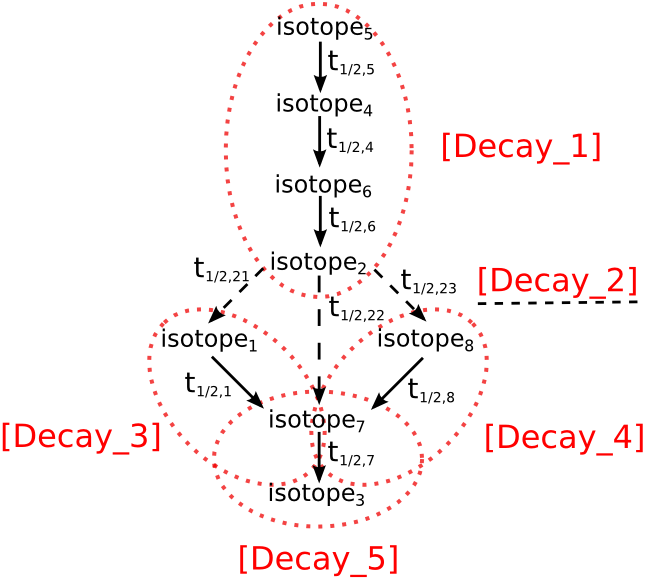
\includegraphics[width = 8cm]{\fig /decay_chain.png}
%  \caption{Decay chain with branches.}
%  \label{pic:dec_branches}
% \end{figure}
% 
% 
% When it comes to a simulation of first order reactions, the kinetic constant is given as an input. 
% The description of a kinetic chemical reaction has obviously two folowing forms
% \[
%   \begin{array}{l}
%     A\xrightarrow{k}B,\\
%     \frac{dc^A}{dt} = -k \cdot c^A.
%   \end{array}
% \]
% The first one description is a standard chemical one. The second equation describes temporal decrease in amount of concentrations of the specie $c^A$. The constant $k$ is so called kinetic constant and for the case of a first order reactions it is equal to so called reaction rate. The order of reaction with just one reactant is equal to the power of $c^A$ in partial diferential reaction.
% 
% For an inclusion of first order reaction into a reaction matrix a half-life needs to be computed from the corresponding kinetic constant $k$. The derivation follows
% \[
%   \begin{array}{l}
%     A\xrightarrow{k} B\\
%     \frac{dc^A}{d\tau} = -k\cdot c_A\\
%     \frac{dc^A}{c^A} = -k\cdot d\tau\\
%     \int\limits_{c^A_0/2}^{c^A_0}\frac{dc^A}{c^A} = -k\cdot\int\limits_{t_{1/2,A}}^{0} d\tau\\
%     \left[ ln c^A\right]_{c^A_0/2}^{c^A_0} = -[k\tau]_{t_{1/2,A}}^{0}\\
%     ln c^A_0 - \ln\frac{c^A_0}{2} = k\cdot t_{1/2,A}\\
% %     c^A (t) = c^A_0\cdot e^{-k\cdot t_{1/2,A}}\\
% %     {\bf substitution} \qquad c^A(t_{1/2,A}) = \frac{1}{2}\cdot c^A_0\\
% %     \frac{1}{2} c^A_0 = c^A_0\cdot e^{-k_1\cdot t_{1/2,A}}\\
%     \ln 2 = k \cdot t_{1/2,A}\\
%     t_{1/2,A} = \frac{ln 2}{k}
%   \end{array}                                                                                                                                                                                                                                                                                                            
% \]
% The matrix ${\bf R}$ is constructed in the same way as for the radioactive
% decay.


% \section{Heat Transfer}
\label{sc:heat}

Under the assumption of thermal equilibrium between the solid and liquid phase, the energy balance equation has the form\footnote{For lower dimensions this form can be derived as in Section \ref{sc:ad_on_fractures} using $w:=\delta\tilde s T$, $u:=T$, $\tn A:=\delta\lambda\tn I$, $\vc b:=\frac{\varrho_l c_l}{\tilde s}\vc w$.}
\[
    \partial_t\left(\delta \tilde s T \right) + \div(\varrho_l c_l T \vc q) - \div(\delta\Lambda\nabla T) = F^T + F^T_C.
\]
The principal unknown is the temperature $T$ [K].
Other quantities are:
\begin{itemize}
\item \hyperA{HeatTransfer-DG-Data::fluid-density}{$\varrho_l$}, \hyperA{HeatTransfer-DG-Data::solid-density}{$\varrho_s$} \units{1}{-3}{} is the density of the fluid and solid phase, respectively.
\item \hyperA{HeatTransfer-DG-Data::fluid-heat-capacity}{$c_l$}, \hyperA{HeatTransfer-DG-Data::solid-heat-capacity}{$c_s$} [J$\mathrm{kg}^{-1}\mathrm{K}^{-1}$] is the heat capacity of the fluid and solid phase, respectively.
\item $\tilde s$ [J$\mathrm{m}^{-3}\mathrm{K}^{-1}$] is the volumetric heat capacity of the porous medium defined as
\[ \tilde s = \hyperA{HeatTransfer-DG-Data::porosity}{\th}\varrho_l c_l + (1-\th)\varrho_s c_s. \]
\item $\Lambda$ [W$\mathrm{m}^{-1}\mathrm{K}^{-1}$] is the thermal dispersion tensor:
\[ \Lambda = \Lambda^{cond} + \Lambda^{disp} \]
\[ \Lambda^{cond} = \left(\th \lambda_l^{cond} + (1-\th)\lambda_s^{cond}\right)\tn I, \]
\[ \Lambda^{disp} = \th \varrho_l c_l|\vc v|\left(\alpha_T\tn I + (\alpha_L-\alpha_T)\frac{\vc v\otimes\vc v}{|\vc v|^2}\right), \]
where \hyperA{HeatTransfer-DG-Data::fluid-heat-conductivity}{$\lambda_l^{cond}$}, \hyperA{HeatTransfer-DG-Data::solid-heat-conductivity}{$\lambda_s^{cond}$} [W$\mathrm{m}^{-1}\mathrm{K}^{-1}$] is the thermal conductivity of the fluid and solid phase, respectively, and \hyperA{HeatTransfer-DG-Data::disp-l}{$\alpha_L$}, \hyperA{HeatTransfer-DG-Data::disp-t}{$\alpha_T$} \units{}{1}{} is the longitudal and transverse dispersivity in the fluid.

\item $F^T$ [J$\mathrm{m}^{-d}\mathrm{s}^{-1}$] represents the thermal source:
\[ F^T = \delta \th F^T_l + \delta (1-\th) F^T_s, \]
\[ F^T_l = f_l^T + \varrho_l c_l \sigma^T_l(T-T_l), \]
\[ F^T_s = f_s^T + \varrho_s c_s \sigma^T_s(T-T_s), \]
where \hyperA{HeatTransfer-DG-Data::fluid-thermal-source}{$f_l^T$}, \hyperA{HeatTransfer-DG-Data::solid-thermal-source}{$f_s^T$} [W$\mathrm{m}^{-3}$] is the density of thermal sources in fluid and solid, respectively, \hyperA{HeatTransfer-DG-Data::fluid-ref-temperature}{$T_l$}, \hyperA{HeatTransfer-DG-Data::solid-ref-temperature}{$T_s$} [K] is a reference temperature and \hyperA{HeatTransfer-DG-Data::fluid-heat-exchange-rate}{$\sigma^T_l$}, \hyperA{HeatTransfer-DG-Data::solid-heat-exchange-rate}{$\sigma^T_s$} \units{}{}{-1} is the heat exchange rate.
\end{itemize}



\paragraph{Initial and boundary conditions.}
At time $t=0$ the temperature is determined by the initial condition
$$ T(0,\vc x) = \hyperA{HeatTransfer-DG-Data::init-temperature}{T_0}(\vc x). $$
Given the decomposition of $\partial\Omega_d$ into $\Gamma_I\cup\Gamma_D\cup\Gamma_N\cup\Gamma_R$ (see Section \ref{sc:transport_model}), we prescribe the following boundary conditions:
\begin{itemize}
\item Dirichlet:
\[ T = \hyperA{HeatTransfer-DG-Data::bc-temperature}{T_D} \mbox{ on }\Gamma_I^+\cup\Gamma_D, \]
\item Homogeneous Neumann:
\[ \left(\varrho_l c_l T \vc q - \delta\Lambda\nabla T\right)\cdot\vc n = 0 \mbox{ on }\Gamma_I^-, \]
\item Neumann:
\[ \left(\varrho_l c_l T \vc q - \delta\Lambda\nabla T\right)\cdot\vc n = \hyperA{HeatTransfer-DG-Data::bc-flux}{f_N} \mbox{ on }\Gamma_N, \]
\item Robin (Newton):
\[ \left(\varrho_l c_l T \vc q - \delta\Lambda\nabla T\right)\cdot\vc n = \hyperA{HeatTransfer-DG-Data::bc-robin-sigma}{\sigma_R}(T-\hyperA{HeatTransfer-DG-Data::bc-temperature}{T_D}) \mbox{ on }\Gamma_R. \]
\end{itemize}






\paragraph{Communication between dimensions.}
Denoting $T_{d+1}$, $T_d$ the temperature in $\Omega_{d+1}$ and $\Omega_d$, respectively, the communication on the interface between $\Omega_{d+1}$ and $\Omega_d$ is described by the quantity
\begin{equation}
  \label{e:inter_dim_flux_heat}
  q^T_{d+1,d} = \sigma^T_{d+1,d} \frac{\delta_{d+1}^2}{\delta_d}2\Lambda_d:\n\otimes\n ( T_{d+1} - T_d) + \begin{cases} \varrho_l c_l q^l_{d+1,d} T_{d+1} & \mbox{ if }q^l_{d+1,d}\ge 0,\\\varrho_l c_l q^l_{d+1,d} \frac{\tilde s_d}{\tilde s_{d+1}} T_d & \mbox{ if } q^l_{d+1,d}<0,\end{cases}
\end{equation}
where
\begin{itemize}
\item $q^T_{d+1,d}$ [W$\mathrm{m}^{-2}$] is the density of heat flux from $\Omega_{d+1}$ to $\Omega_d$,
\item \hyperA{HeatTransfer-DG-Data::fracture-sigma}{$\sigma^T_{d+1,d}$} \units{}{}{} is a transition parameter.
Its value determines the exchange of energy between dimensions due to temperature difference.
In general, it is recommended to leave the default value $\sigma^T=1$ or to set $\sigma^T=0$ (when exchange is due to water flux only).
\item $q^l_{d+1,d}=\vc q_{d+1}\cdot\vc n$ is the water flux from $\Omega_{d+1}$ to $\Omega_d$.
\end{itemize}
The communication between dimensions is incorporated as the total flux boundary condition for the problem on $\Omega_{d+1}$:
\begin{equation}
\label{e:heat_FC}
\left(\varrho_l c_l T \vc q - \delta\Lambda\nabla T\right)\cdot\vc n = q^T
\end{equation}
and a source term in $\Omega_d$:
\begin{equation}
F^T_{C3} = 0,\quad
F^T_{C2} = q^T_{32},\quad
F^T_{C1} = q^T_{21}.
\end{equation}




\paragraph{Energy balance.}
The heat equation satisfies the balance of energy in the following form:
$$ e(0) + \int_0^t s(\tau) \,d\tau - \int_0^t f(\tau) \,d\tau = e(t) $$
for any instant $t$ in the computational time interval.
Here
$$ e(t) := \sum_{d=1}^3\int_{\Omega^d}(\delta \tilde s T)(t,\vc x)\,d\vc x, $$
$$ s(t) := \sum_{d=1}^3\int_{\Omega^d}F_S^T(t,\vc x)\,d\vc x, $$
$$ f(t) := \sum_{d=1}^3\int_{\partial\Omega^d}\left(\varrho_l c_l T\vc q - \delta\Lambda\nabla T\right)(t,\vc x)\cdot\vc n \,d\vc x $$
is the energy [J], the volume source [J$\mathrm{s}^{-1}$] and the energy flux [J$\mathrm{s}^{-1}$] at time $t$, respectively.
The energy, flux and source on every geometrical region is calculated at each computational time step and the values together with the control sums are written to the file \texttt{energy\_balance.txt}.







% \chapter{Numerical Methods}
% % TODO: Update numerical topics
% \section{Diagonalized Mixed-Hybrid Method}
\def\mr{\mathring}
Model of flow described in section \ref{sec:darcy_flow} is solved by
the mixed-hybrid formulation (MH) of the finite element method.
As in the previous chapter, let
$\tau$ be the time step and $\mathcal T_d$ a regular simplicial partition of $\Omega_d$, $d=1,2,3$.
Denote by $\vc W_d(T_d)\subset \vc H(div,T_d)$
 the space of Raviart-Thomas functions of order zero ($RT_0$) on an element $T_d\in 
\mathcal T_d$.
We introduce the following spaces:
\[
    \vc W =  \vc W_1 \times \vc W_2 \times \vc W_3,\quad
    \vc W_d = \prod_{T_d\in \mathcal T_d} \vc W_d(T_d),
\]
\begin{equation}
Q=Q_{1}\times Q_{2}\times Q_{3},
\quad
Q_{d}=L^{2}\left(  \Omega_{d}\right).
\end{equation}
For every $T_d\in \mathcal T_d$ we define the auxiliary space of values on interior sides of $T_d$:
\begin{equation}
    \mr Q(T_d)=\left\{  \mr q\in 
    L^{2}(\partial T_d \setminus  \partial\Omega_d^D):
    \mr q =\vc w\cdot \vc n|_{\partial T_d},
    \vc w\in\vc W_d%
    \right\}.
\end{equation}
Further we introduce the space of functions defined on interior sides that do not coincide with elements of the lower dimension:
\begin{equation}
    \mr Q_d=\Big\{
        \mr q\in\prod_{T \in \mathcal T_d} \mr Q(T);
        \ \mr q|_{\partial T}=\mr q|_{\partial \tilde T}%
        \quad\text{on the side }F=\partial T\cap\partial \tilde T
        \quad\text{ if }F\cap\Omega_{d-1}=\emptyset
    \Big\}.
\end{equation}
Finally we set $\mr Q = \mr Q_1 \times \mr Q_2 \times \mr Q_3$.

The \emph{mixed-hybrid method} for the unsteady Darcy flow reads as follows.
We are looking for a trio $(\mathbf{u},h,\mr h)  
\in \vc W\times Q\times\mr Q$ which satisfies the saddle-point problem:
\begin{align}
    a(\vc u,\vc v)  +b(\vc v, p) + \mr b(\vc v, \mr p)
        &=\langle g,\vc v \rangle, \qquad\forall \vc v\in \vc W,
        \label{eq:hybrid-frac-1}\\
    b(\vc u, q ) + \mr b( \vc u, \mr q) - c(p, \mr p, q, \mr q)
        &= \langle f, (q,\mr q) \rangle,
        \qquad\forall q\in Q,\ \mr q\in \mr Q, 
        \label{eq:hybrid-frac-2}
\end{align}
where
\begin{align}
    \label{eq:weak_term_a}
    a(\vc u, \vc v) &= \sum_{d=1}^{3}\sum_{T\in \mathcal T_d}
    \int_{T} \frac{1}{\delta_{d}}\tn K_{d}^{-1} 
    \vc u_d\cdot \vc v_d\,dx,
    \\
    \label{eq:weak_term_b}
    b(\vc u, q)  &= -\sum_{d=1}^{3}\sum_{T\in \mathcal T_d}
    \int_{T} q_d\,\div \vc u_d\,dx,
    \\
    \label{eq:weak_term_bf}
    \mr b(\vc u, \mr q)   &= \sum_{d=1}^{3}\sum_{T\in \mathcal T_d}
    \int_{\partial T\setminus\partial\Omega_{d}}
        \mr q|_{\partial T} ( \vc u_d\cdot\vc n)\,ds,
    \\
    \label{eq:weak_term c}
    c(h, \mr h, q, \mr q) &= c_f(h, \mr h, q, \mr q) 
    + c_t(h, \mr h, q, \mr q) + c_R(\mr h, \mr q)
    \\
    c_f(h, \mr h, q, \mr q)&=\sum_{d=2,3}\sum_{T\in \mathcal T_d}
        \int_{\partial T \cap\Omega_{d-1}} \sigma_{d} 
        (p_{d-1} - \mr p_d)(q_{d-1} - \mr q_d)\,ds
    \\
    c_t(h, \mr h, q, \mr q)&= \sum_{d=1}^{3}\sum_{T\in \mathcal T_d}
        \int_{T} \frac{\delta_d S_d}{\tau} h_d q_d\,dx,
    \\    
    c_R(\mr h, \mr q)&=
    \int_{\partial T\setminus\partial\Omega_{d}}
        \sigma_d^R\, h_d \mr q_d \,ds,
    \\
    \langle g, \vc v \rangle  & =
    -\sum_{d=1}^{3}\sum_{T\in\mathcal T_d}
    \int_{\partial T\cap\partial\Omega_N} 
        p_d^D\, (\vc v \cdot \vc n)  \,ds,
    \\
    \langle f, q \rangle  &=
    -\sum_{d=1}^{3}\int_{\Omega_d} \delta_{d}\,f_d\,q_{d}\,dx,
    \\
        &\phantom{=}+
    \sum_{d=1}^{3}\sum_{T\in\mathcal T_d}
    \int_{\partial T\cap\partial\Omega_N} 
        q_d^N \mr q_d - \sigma_d^R\, h_d^R \mr q_d\,ds
    \\
        &\phantom{=}-c_t(\tilde h, \mr{\tilde{h}}, q, \mr q).
    \label{eq:weak_term_f}%    
\end{align}
All quantities are meant in time $t$, only $\tilde h$ is the pressure head in time $t-\tau$.

The advantage of the mixed-hybrid method is that the set of equations $\eqref{eq:hybrid-frac-1} - 
\eqref{eq:hybrid-frac-2}$ can be reduced by eliminating the unknowns $\vc u$ and $q$
to a sparse positive definite system for $\mr q$.
This equation can then be efficiently solved using a~preconditioned conjugate gradient method.
Unfortunately, it appears that the resulting system does not satisfy the discrete maximum principle
 which in particular for short time steps $\tau$ can lead to unphysical oscillations.
One possible solution is the diagonalization of the method (lumped mixed-hybrid method, LMH)
 proposed in \cite{younes_2006}.
This method was implemented in Flow123d as well.
It consists in replacing the form $c_t$ by
\[
    c_t(h, \mr h, q, \mr q)= \sum_{d=1}^{3}\sum_{T\in \mathcal T_d}
        \sum_{i=1}^{d+1} \alpha_{T,i} \abs{T} \frac{\delta_d S_d}{\tau} 
        \left(\mr h|_{S_{T,i}}\,  \mr q|_{S_{T,i}}\right),
\]
and the source term $\sum_{d=1}^{3}\int_{\Omega_d} \delta_{d}\,f_d\,q_{d}\,dx$ by
\[
    \sum_{d=1}^{3}\sum_{T\in \mathcal T_d}
        \sum_{i=1}^{d+1} \alpha_{T,i} \abs{T} \delta_d f_d\,
        \mr q|_{S_{T,i}},
\]
where $\abs{T}$ is the size of an element $T$, $S_{T,i}$ is the $i$-th side of $T$, and 
$\mr h|_{S_{T,i}}$ is the degree of freedom on the side $S_{T,i}$. 
Weights $\alpha_{T,i}$ can be chosen to be $1/(d+1)$. 
After solving the set of equations it is necessary to modify the velocity field $\vc u$
 by adding the time term.
This modified system already satisfies the discrete maximum principle
 and does not produce oscillations.
Figure \ref{fig:LMH} shows a comparison of the results
 using conventional MH scheme and LMH scheme.
At the MH scheme one can observe oscillations in the wavefront
 where the minimum value is significantly less than zero.

\begin{figure}
    \begin{center}
       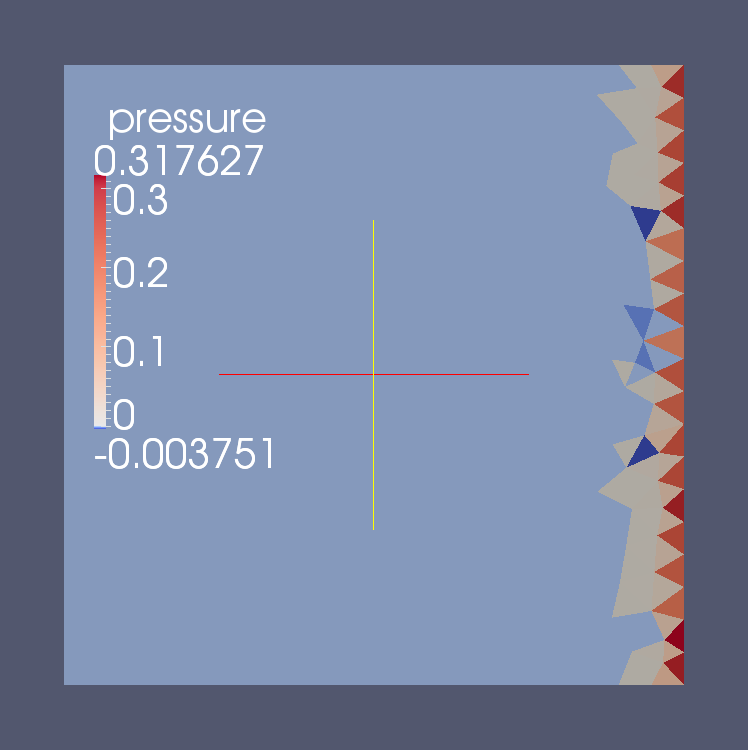
\includegraphics[width=0.4\textwidth]{figures/MH.png}
       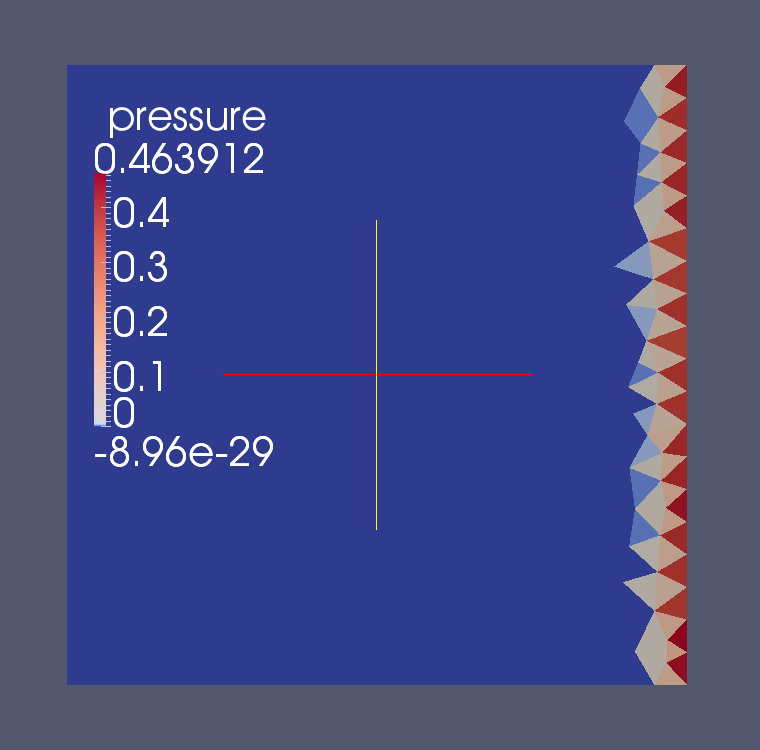
\includegraphics[width=0.405\textwidth]{figures/LMH.png}        
    \end{center}
    \caption{Comparison of MH (left) and LMH scheme (right), $\tau=10^{-4}$.}
    \label{fig:LMH}
\end{figure}



% %%%%%%%%%%%%%%%%%%%%%%%%%%%%%%%%%%%%%%%%%%%%%%%%%%%%%%%%%%%%%%%%%%%%%
\section{Discontinuous Galerkin Method}
\label{sc:dg}

\def\Eh{\mathcal E_d}       % edges of \Th
\def\Ehb{\mathcal E_{d,B}}  % edges of \Th on boundary
\def\Ehcom{\mathcal E_{d,C}}         % edges of \Th on interface with lower dimension
\def\Ehdir{\mathcal E_{d,D}}         % Dirichlet edges of \Th
\def\Ehint{\mathcal E_{d,I}}       % interior edges of \Th
\def\Ehneu{\mathcal E_{d,N}}         % Neumann or Robin edges of \Th
\def\Ngh{\mathcal N_d}
\def\avg#1{\left\{#1\right\}}
\def\jmp#1{[#1]}
\def\wavg#1#2#3{\avg{#1}_{#2,#3}^\omega}
\def\Td{\mathcal T_d}


Models for solute transport and heat transfer described in sections \ref{sc:transport_model} and \ref{sc:heat} are collectively formulated
 as a system of abstract advection-diffusion equations on domains $\Omega_d$, $d=1,2,3$,
 connected by communication terms.
Consider for $d=1,2,3$ the equation 
\begin{subequations}
 \label{eq:abstr_system}
 \begin{equation}
  \partial_t u_d + \div(\vc b u_d) - \div(\tn A\nabla u_d) = f^0+f^1(u^S-u_d) + q(u_{d+1},u_d) \mbox{ in }(0,T)\times\Omega_d
 \end{equation}
 with initial and boundary conditions
 \begin{align}
  u_d(0,\cdot) &= u^0 &&\mbox{ in }\Omega_d,\\
  \label{eq:bc_abstr_dir} u_d &= u^D &&\mbox{ on }(0,T)\times\Gamma^D_d,\\
  \label{eq:bc_abstr_neu} (\vc b u_d-\tn A\nabla u_d)\cdot\vc n &= f^N + \sigma^R(u_d - u^D) &&\mbox{ on }(0,T)\times\Gamma^N_d,\\
  (\vc b u_d-\tn A\nabla u_d)\cdot\vc n &= q(u_d,u_{d-1}) &&\mbox{ on } (0,T)\times\Gamma^C_d,
 \end{align}
 where
 \[ \Gamma^C_d:=\overline\Omega_d\cap\overline\Omega_{d-1}. \]
 The communication term $q(u_{d+1},u_d)$ has the form
 \begin{equation}
 \label{eq:com_term_abstr_system}
  q(u_{d+1},u_d) =
  \begin{cases}
      \alpha u_{d+1} + \beta u_d
    & \mbox{ in }\Gamma^C_{d+1},~d=1,2,\\ 0
    & \mbox{ on }\Omega_d\setminus\Gamma^C_{d+1},~d=1,2,\mbox{ and for }d=0,3.
  \end{cases}
 \end{equation}
\end{subequations}
System \eqref{eq:abstr_system} is spatially discretized by the discontinuous Galerkin method
 with weighted averages,
 which was derived for the case of one domain in \cite{ern_stephansen_zunino}
 (for a posteriori estimate see \cite{ern2010guaranteed}).
For time discretization we use the implicit Euler method.

Let $\tau$ denote the time step.
For a regular splitting $\Td$ of $\Omega^d$, $d=1,2,3$, into simplices we define the following sets of element sides:
\begin{align*}
 &\Eh &&\mbox{sides of all elements in $\Td$ (i.e. triangles for $d=3$, lines for $d=2$ and nodes for $d=1$)},\\
 &\Ehint &&\mbox{interior sides (shared by 2 or more $d$-dimensional elements)},\\
 &\Ehb &&\mbox{outer sides (belonging to only one element)},\\
 &\Ehdir(t) &&\mbox{sides, where the Dirichlet condition \eqref{eq:bc_abstr_dir} is given},\\
 &\Ehneu(t) &&\mbox{sides, where the Neumann or Robin condition \eqref{eq:bc_abstr_neu} is given},\\
 &\Ehcom &&\mbox{sides coinciding with $\Gamma^C_d$}.
\end{align*}
For an interior side $E$ we denote by $\Ngh(E)$ the set of elements that share $E$ (notice that 1D and 0D sides can be shared by more than 2 elements).
For an element $T\in\Ngh(E)$ we denote $q_T:=(\vc b\cdot\vc n)_{|T}$ the outflow from $T$,
and define $\Ngh^-(E):=\{T\in\Ngh(E)\where q_T\le 0\}$, $\Ngh^+(E):=\{T\in\Ngh(E)\where q_T>0\}$
the sets of all outflow and inflow elements, respectively.
For every pair $(T^+,T^-)\in \Ngh^+(E)\times\Ngh^-(E)$ we define the flux from $T^+$ to $T^-$ as
$$ q_{T^+\to T^-} := \frac{q_{T^+} q_{T^-}}{\sum_{T\in\Ngh^-(E)}{q_T}}.$$
We select arbitrary element $T_E\in\Ngh(E)$ and define $\n_E$ as the the unit outward normal vector to $\partial T_E$ at $E$.
The jump in values of a function $f$ between two adjacent elements $T_1,T_2\in\Ngh(E)$ is defined by $\jmp{f}_{T_1,T_2}=f_{|T_{1|E}}-f_{|T_{2|E}}$,
 similarly we introduce the average $\avg{f}_{T_1,T_2}=\frac12(f_{|T_{1|E}} + f_{|T_{2|E}})$
 and a weighted average $\wavg{f}{T_1}{T_2}=\omega f_{|T_{1|E}} + (1-\omega) f_{|T_{2|E}}$.
The weight $\omega$ is selected in a specific way (see \cite{ern_stephansen_zunino})
 taking into account the possible inhomogeneity of the tensor $\tn A$.

% Let us fix one substance and the space dimension $d$.
For every time step $t_k=k\tau$ we look for the discrete solution $u^{k}=(u_1^{k},u_2^{k},u_3^{k})\in V$, where
$$ V=\prod_{d=1}^3 V_d \quad\mbox{ and }\quad V_d = \{v:\overline{\Omega^d}\to\R\where v_{|T}\in P_p(T)~\forall T\in\Td\} $$
are the spaces of piecewise polynomial functions of degree at most $p$ on elements $\Td$,
 generally discontinuous on interfaces of elements.
The initial condition for $u_d^{0}$ is defined as the $L^2$-projection of $u^0$ to $V_d$.
For $k=1,2,\ldots$, $u^{k}$ is given as the solution of the problem
\begin{equation*}
 \frac1\tau\sc{u^{k}-u^{k-1}}{v}_{V} + a^{k}(u^{k},v) = b^{k}(v) \quad \forall v\in V.
\end{equation*}
Here $\sc{f}{g}_{V}=\sum_{d=1}^d\sc{f}{g}_{\Omega^d}$, $\sc{f}{g}_{\Omega^d}=\int_{\Omega^d} f g$,
 and forms $a^{k}$, $b^{k}$
 are defined as follows:
\begin{multline}
\label{eq:df_ak_abstr_sys}
  a^{k}((u_1,u_2,u_3),(v_1,v_2,v_3))\\
   = \sum_{d=1}^3\bigg( a^{k}_d(u_d,v_d)
    - \sc{q(u_{d+1},u_d)}{v_d}_{\Omega^d}
    - \sum_{E\in\Ehcom^d(t_k)}\sc{q(u_d,u_{d-1})}{v_d}_E \bigg),
\end{multline}
\begin{equation}
\label{eq:df_bk_abstr_sys}
b^{k}((v_1,v_2,v_3)) = \sum_{d=1}^3 b^{k}_d(v_d), \mbox{\hspace{11.7cm}}
\end{equation}
\begin{align*}
 a^{k}_d(u,v) = &\sc{\tn A\nabla u}{\nabla v}_{\Omega^d}
 - \sc{\vc b u}{\nabla v}_{\Omega^d} + \sc{f^1 u}{v}_{\Omega^d}\\
 &- \sum_{E\in\Ehint^d}\sum_{\substack{T_1,T_2\in\Ngh(E)\\T_1\neq T_2}}\bigg(\sc{\wavg{\tn A\nabla u}{T_1}{T_2}\cdot\n_E}{\jmp{v}_{T_1,T_2}}_E + \Theta\sc{\wavg{\tn A\nabla v}{T_1}{T_2}\cdot\n_E}{\jmp{u}_{T_1,T_2}}_E \\
 &- \gamma_E\sc{\jmp{u}_{T_1,T_2}}{\jmp{v}_{T_1,T_2}}_E \bigg)
 - \sum_{E\in\Ehint^d}\sum_{\substack{T^+\in\Ngh^+(E)\\T^-\in\Ngh^-(E)}}\sc{q_{T^+\to T^-}\avg{u}_{T^+,T^-}}{\jmp{v}_{T^+,T^-}}_E\\
%  & + \sum_{E\in\Ehb^d}\sc{\vc b\cdot\n u}{v}_E
 &+ \sum_{E\in\Ehdir^d(t_k)}\bigg(\gamma_E\sc{u}{v}_E + \sc{\vc b\cdot\n u}{v}_E - \sc{\tn A\nabla u\cdot\vc n}{v}_E - \Theta\sc{\tn A\nabla v\cdot\vc n}{u}_E\bigg)\\
 &+ \sum_{E\in\Ehneu^d(t_k)}\sc{\sigma^R u}{v}_E,\\
% \end{multline*}
% 
% \begin{equation*}
 b^{k}_d(v) = &\sc{f^0+f^1 u^S}{v}_{\Omega^d} + \sum_{E\in\Ehdir^d(t_k)}\bigg(\gamma_E\sc{u^D}{v}_E - \Theta\sc{u^D}{\tn A\nabla v\cdot\vc n}_E\bigg)\\
 & + \sum_{E\in\Ehneu^d(t_k)}\sc{\sigma^R u^D-f^N}{v}_E.
\end{align*}
The Dirichlet condition is here enforced by a penalty with an arbitrary parameter $\gamma_E>0$;
 its value influences the level of solution's discontinuity.
For $\gamma_E\to+\infty$ we obtain asymptotically (at least formally) the finite element method.
The constant $\Theta$ can take the values $-1$, $0$ or $1$,
 where $-1$ corresponds to the nonsymetric, $0$ to the incomplete and $1$ to the symetric variant of the discontinuous Galerkin method.




\section{Finite Volume Method for Convective Transport}

In the case of the purely convective solute transport ($\tn D=0$), problem \eqref{eq:abstr_system} is replaced by:
\begin{subequations}
 \label{eq:abstr_system_conv}
 \begin{align}
  \partial_t u_d + \div(\vc b u_d) &= f^0+f^1(u^S-u_d) + q(u_{d+1},u_d) &&\mbox{ in }(0,T)\times\Omega_d,\\
  u_d(0,\cdot) &= u^0 &&\mbox{ in }\Omega_d,\\
  \label{eq:bc_abstr_neu} (\vc b\cdot\vc n) u_d &= (\vc b\cdot\vc n) u^D &&\mbox{ on }\Gamma_d^I,
 \end{align}
\end{subequations}
 where
 \[ \Gamma_d^I:=\{(t,\vc x)\in(0,T)\times\partial\Omega_d\where \vc b(t,\vc x)\cdot\vc n(\vc x)<0\}. \]
 The communication term $q(u_{d+1},u_d)$ has the same structure as in \eqref{eq:com_term_abstr_system}.

The system is discretized by the cell-centered finite volume method combined with the explicit Euler time discretization.
Using the notation of Section \ref{sc:dg}, we consider the space $V$ of piecewise constants on elements and define the discrete problem:
\begin{equation*}
 \frac1\tau\sc{u^{k}-u^{k-1}}{v}_{V} + a^{k-1}(u^{k-1},v) = b^{k-1}(v) \quad \forall v\in V,
\end{equation*}
where the forms $a^k$ and $b^k$ are defined in \eqref{eq:df_ak_abstr_sys}-\eqref{eq:df_bk_abstr_sys} and $a^k_d$, $b^k_d$ now have simplified form:
\begin{align*}
 a^{k}_d(u,v) = & -\sum_{T_i\in\Td}\left(\sc{(\vc b\cdot\vc n)^+u}{v}_{\partial T_i} + \sum_{T_j\in\Td}\sc{q_{T_j\to T_i}u}{v}_{\partial T_i\cap\partial T_j} \right),\\
 b^{k}_d(v) = &\sc{f^0+f^1(u^S-u^{k-1}_d)^+}{v}_{\Omega^d} + \sum_{T_i\in\Td}\sc{(\vc b\cdot\vc n)^-u^D}{v}_{\partial T_i\cap\partial\Omega_d}.
\end{align*}
The above formulation corresponds to the upwind scheme, ideal mixing in case of multiple elements sharing one side, and explicit treatment of linear source term.

% \input convection


% \section{Solution Issues for Reaction Term}

% \input{decay}

\subsection{Dual Porosity} 
\label{sec:num_dual_porosity}

The analytic solution of the system of differential equations \eqref{eq:odes_dual_por} at the time $t$ with initial conditions $c_m(0)$ and $c_i(0)$ is
\begin{align}
     c_m(t) &= (c_m(0) - c_a(0)) \exp\left(- D_{dp}\left(\frac{1}{\vartheta_m} + \frac{1}{\vartheta_i}\right) t \right) + c_a(0), 
     \label{eqn:dual_porosity_anal1}\\
     c_i(t) &= (c_i(0) - c_a(0)) \exp\left(- D_{dp}\left(\frac{1}{\vartheta_m} + \frac{1}{\vartheta_i}\right) t \right) + c_a(0),
     \label{eqn:dual_porosity_anal2}
\end{align}
where $c_a$ is the weighted average
\[
  c_a = \frac{\vartheta_m c_m + \vartheta_i c_i}{\vartheta_m + \vartheta_i}.
\]

If the time step is large, we use the analytic solution to compute new values of concentrations. 
Otherwise, we replace the time derivatives in \eqref{eqn:dual_porosity_ode1} and \eqref{eqn:dual_porosity_ode2} 
by first order forward differences and we get the classical Euler scheme
\begin{align}
  c_m(t^+) = \frac{D_{dp} \Delta t}{\vartheta_m}(c_i(t) - c_m(t)) + c_m(t), \\
  c_i(t^+) = \frac{D_{dp} \Delta t}{\vartheta_i}(c_m(t) - c_i(t)) + c_i(t), \\
\end{align}
where $\Delta t = t^+ - t$ is the time step. 

The condition on the size of the time step is derived from the Taylor expansion of 
\eqref{eqn:dual_porosity_anal1} or \eqref{eqn:dual_porosity_anal2}, respectively. We neglect the higher order 
terms and we want the second order term to be smaller than the given \hyperA{DualPorosity::scheme-tolerance}{scheme tolerance} 
$tol$, relatively to $c_a$,
\begin{equation}
  (c_m(0) - c_a(0))
  \frac{ D_{dp}^2 (\Delta t)^2 \left(\frac{\vartheta_m + \vartheta_i}{\vartheta_m \vartheta_i}\right)^2}{2}
  \frac{1}{c_a} \leq tol. \\
\end{equation}
We then transform the above inequation into the following condition which is tested in the program
\begin{equation} \label{eqn:euler_scheme_condition}
  \max(|c_m(0) - c_a(0)|, |c_i(0) - c_a(0)|) \leq 
  2 c_a \left(\frac{\vartheta_m \vartheta_i}{D_{dp} \Delta t (\vartheta_m + \vartheta_i)}\right)^2 tol. \\
\end{equation}
If the inequation \eqref{eqn:euler_scheme_condition} is not satisfied, then the analytic 
solution is used.


\subsection{Equilibrial Sorption}
\label{sec:num_sorp_math}

Let us now describe the actual computation of the sorption model.
To solve \eqref{eq:nonlin_sorption} iteratively, it is very important to define the interval where 
to look for the solution (unknown $c_l$), see Figure \ref{fig:sorpce}. The lower bound is $0$ (concentration can not reach negative values). 
The upper bound is derived using a simple mapping. Let us suppose limited 
\hyperA{Sorption::solubility}{solubility} of the selected transported substance and let us denote the 
limit $\bar{c}_l$. We keep the maximal "total mass" 
$\bar{c}_T= \mu_l\cdot \bar{c}_l + \mu_s\cdot f(\bar{c}_l)$, but we dissolve all the mass to get 
maximal $c_l^{max} > \bar{c}_l$. That means $c_s = 0$ at this moment. We can slightly enlarge the interval by setting the upper bound equal to 
$c_l^{max} + const_{small}$.

\begin{figure}[ht!]
 \centering
 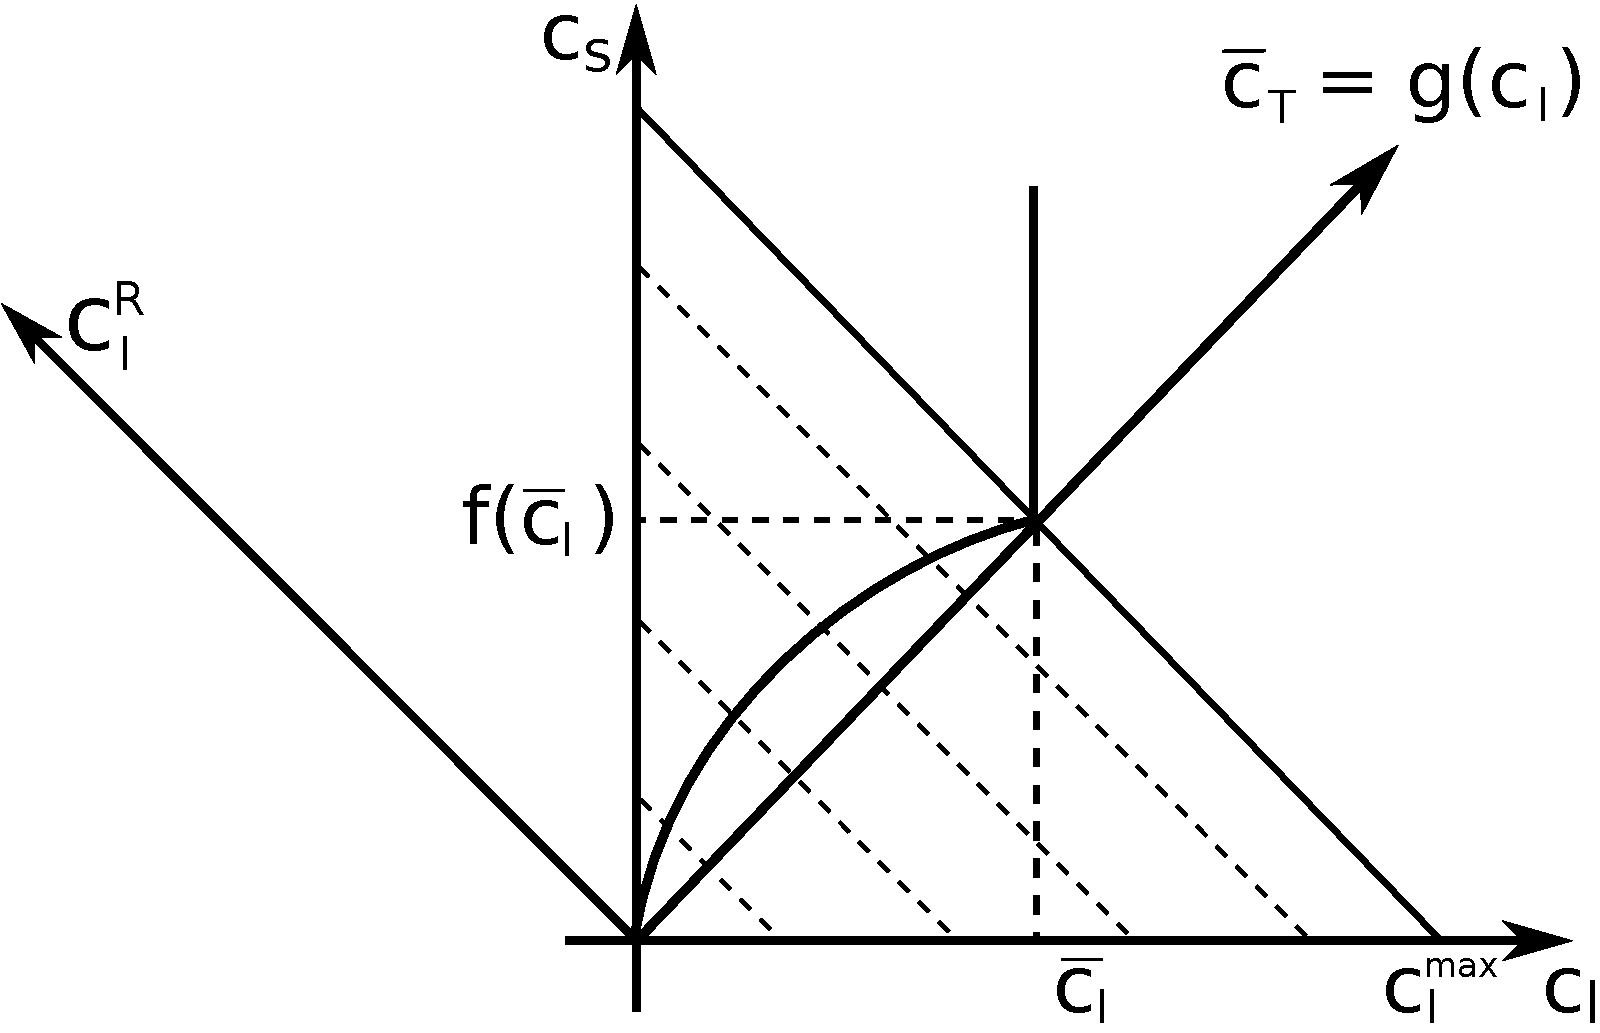
\includegraphics[width = 0.75\textwidth]{\fig/sorpce.pdf}
 \caption{Sorption in combination with limited solubility.}
 \label{fig:sorpce}
\end{figure}


To approximate the equation \eqref{eq:nonlin_sorption} using interpolation, we need to prepare the set of values 
which represents $[c_l, f(c_l)]$, with $c_l$ equidistantly distributed in transformed (rotated and rescaled) 
coordination system at first. The construction process of the interpolation table follows.
\begin{enumerate}
 \item Maximal ``total mass'' $\bar{c}_T = \mu_l\cdot \bar{c}_l + \mu_s\cdot f(\bar{c}_l)$ is computed.
 \item Total mass step is derived $mass\_step = \bar{c}_T/n\_steps$. $n\_steps$ is the number of
       \hyperA{Sorption::substeps}{substeps}.
 \item Appropriate $c_T^j = (mass\_step\cdot j)/\mu_l,~j\in \{0,\ldots, n\_steps\}$ are computed. 
 \item The equations $\mu_l \cdot c_T^j = \mu_l\cdot c_l^j + \mu_s\cdot f(c_l^j)~j\in \{0,\ldots, n\_steps\}$ are solved 
       for $c_l^j$ as unknowns. The solution is the set of ordered couples (points) 
       $[c_l^j,f(c_l^j)],~j\in\{0,\ldots,n\_steps\}$.
\end{enumerate}
After the computation of $\{[c_l^j,f(c_l^j)]\}$, we transform these coordinates to the system where the total mass is 
an independent variable. This is done by multiplication of precomputed points using the transformation matrix ${\bf A}$:
\begin{equation}
 \begin{array}{l}
  \vec{c}\,^R = {\bf A}\cdot\vec{c}\\
  \left[\begin{array}{c} c_l^{R,j}\\ c_s^{R,j} \end{array}\right] = 
  \left[\begin{array}{cc}
    \vartheta\cdot \rho_w & M_s(1 - \vartheta)\rho_R\\
    -M_s(1 - \vartheta)\rho_R & \vartheta\cdot \rho_w
  \end{array}\right]\cdot
  \left[\begin{array}{c} c_l^j\\ c_s^j \end{array}\right]\\
  j\in\{0,\ldots,n\_steps\}
 \end{array}
 \label{eq:transf_mat}
\end{equation}

The values $c_l^{R,j}$ are equidistantly distributed and there is no reason to save them, but the values 
$c_s^{R,j}$ are stored in onedimensional interpolation table.

Once we have the interpolation table, we can use it for projecting the transport results ${[c_l,c_s]}$ on the 
isotherm under consideration. Following steps must be taken.
\begin{enumerate}
 \item Achieved concentrations are transformed to the coordinate system through multiplication with the 
       matrix ${\bf A}$, see \eqref{eq:transf_mat}.
 \item Transformed values are interpolated.
 \item The result of interpolation is transformed back. The backward transformation consists of multiplication 
       with ${\bf A}^T$ which is followed by rescaling the result. Rescaling the result is necessary because  
       ${\bf A}$ is not orthonormal as it is shown bellow.
 \[
 \begin{array}{l}
 {\bf A}^T\cdot{\bf A} =
  \left((\vartheta - 1)^2\cdot M_s^2\cdot \rho_R^2 + \vartheta^2\cdot \rho_w^2\right)\cdot\left[\begin{array}{cc}
    1 & 0\\
    0 & 1
  \end{array}\right]
  \end{array}
 \]
\end{enumerate}


% \subsection{Limited Solubility}\label{subsec:lim_solub}
\paragraph{Limited solubility.} When $\mu_l\cdot c_l + \mu_s\cdot f(c_l) > \mu_l\cdot \bar{c}_l + \mu_s\cdot f(\bar{c}_l)$, neither iterative 
solver nor interpolation table is used. The aqueous concentration is set to be $\bar{c}_l$ and sorbed 
concentration is computed $c_s = (\mu_l\cdot c_l + \mu_s\cdot f(c_l) - \mu_l\cdot \bar{c}_l)/\mu_s$.

\subsection{System of Linear Ordinary Differential Equations}
\label{sec:num_slode}

A system of linear ordinary differential equations (ODE) appears in several places in the model. We provide 
several \hyperA{IT::LinearODESolver}{solvers} which we shall brielfy describe in this section. Let us denote 
the ODE system
\[
  \partial_t \vc c(t) = \mathbf{A}(t) \vc{c}(t) + \vc{b}(t).
\]

\paragraph{Semi-analytic solution.}
A \hyperA{IT::LinearODEAnalytic}{semi-analytic} solution can be obtained in special cases due to the physical nature of the problem.
The problem can be then solved only by a~matrix multiplication $\vc c(t+\Delta t) = \mathbf{R} \vc{c}(t)$. 
This is used in case of radioactive decays and first order kinetic reactions.

The right hand side $\vc{b}$ is zero and $\mathbf{A}$ is constant. The assumption is made that the equations 
are independent during one time step. Each quantity $c_i$ (concentration in this case) is decreased 
by $e^{a_{ii} \Delta t}$ (supposing negative diagonal) during time step $\Delta t$. The decrement $\left( 1-e^{a_{ii} \Delta t} \right)$
is then distributed among other quantities according to the given fraction.

In case of radioactive decays and first order reactions, the elements of the solution matrix $\mathbf{R}$ are
\begin{eqnarray*}
     r_{ii} &=& e^{-k_i \Delta t}, \\
     r_{ji} &=& \left( 1-e^{-k_i \Delta t} \right) b_{ji} \frac{M_j}{M_i},
\end{eqnarray*}
where $b_{ji}$ is the branching ratio of $i$-th reactant (or radionuclide) and $\frac{M_j}{M_i}$ is 
the fraction of molar masses.
The expressions $b_{ji} \frac{M_j}{M_i}$ are then obtained from the system matrix by dividing 
$-\frac{a_{ji}}{a_{ii}}$. See the system matrix entries in \eqref{eqn:reaction_system_entries}.

The assumption (equations independence) is adequate when a very small time step is applied. This will then lead 
to huge amount of evaluations of the exponential functions which can be expensive, so other numerical methods 
might be more appropriate. When the time step is large then the assumption is inadequate.

On the other hand, if the time step is constant (for significantly large number of time steps), we get the
solution cheaply just by matrix multiplication, because the matrix $\mathbf{R}$ is constant.


\paragraph{Pad{\' e} approximant.}
For homogenous systems with constant matrix $\mathbf{A}$, we can use \hyperA{IT::PadeApproximant}{Pad{\' e} approximation} 
to find the solution. This method finds a rational function whose power series agrees with a power series expansion of 
a given function to the highest possible order (e.g. in \cite{press_numerical_1992}).
Let
\[
  f(t) = \sum\limits_{j=0}^{\infty} c_j t^j = \sum\limits_{j=0}^{\infty} \frac{1}{n!}f^{(j)}(t_0)
\]
be the function being approximated and its power series given by Taylor expansion about $t_0$.
Then the rational function
\begin{equation} \label{eqn:pade_approximant}
R_{mn}(t) = \frac{P_m(t)}{Q_n(t)} = \frac{\sum\limits_{j=0}^{m} p_jt^j}{\sum\limits_{j=0}^{n} q_jt^j},
\end{equation}
which satisfies 
\begin{equation} \label{eqn:pade_coef_equations}
f(t)\approx \sum\limits_{j=0}^{m+n} c_j t^j = R_{mn}(t),
\end{equation}
% \begin{equation} \label{eqn:pade_coef_equations}
% \sum\limits_{j=0}^{m+n} c_jt^j \sum\limits_{j=0}^{m} q_jt^j = \sum\limits_{j=0}^{n} p_jt^j,
% \end{equation}
is called Pad{\' e} approximant. From \eqref{eqn:pade_coef_equations}, we obtain $m+n+2$ equations for
coefficients of the nominator $P_m$ (polynomial of \hyperA{PadeApproximant::nominator-degree}{degree} $m$) and 
the denominator $Q_n$ (polynomial of \hyperA{PadeApproximant::denominator-degree}{degree} $n$). We also see that the error 
of the approximation is $O(t^{m+n+1})$. By convention, the denominator is normalized such that $q_0=1$.

Now, we consider the solution of our ODE system in a form $\vc{c}(t)=e^{\mathbf{A}t}\vc{c}(0)$. We shall 
approximate the matrix exponential function using a matrix form of \eqref{eqn:pade_approximant}. 
For exponential functions, there are known coeffficients of the nominator and denominator:
% http://mathoverflow.net/questions/41226/pade-approximant-to-exponential-function
% http://www.math.vanderbilt.edu/~esaff/texts/144.pdf
% https://www-sop.inria.fr/apics/anap03/PadeTalk.pdf
\begin{eqnarray}
  \mathbf{P}_m(\mathbf{A}t) &=& \sum\limits^{m}_{j=0}\frac{(m+n-j)!m!}{(m+n)!j!(m-j)!} (\mathbf{A}t)^j, \\
  \mathbf{Q}_n(\mathbf{A}t) &=& \sum\limits^{n}_{j=0} (-1)^j \frac{(m+n-j)!n!}{(m+n)!j!(n-j)!} (\mathbf{A}t)^j.
\end{eqnarray}
Finally, we can write the solution at time $t+\Delta t$
\begin{equation} \label{eqn:pade_solution}
\vc{c}(t+\Delta t) = \frac{\mathbf{P}_m(\mathbf{A}\Delta t)} {\mathbf{Q}_n(\mathbf{A}\Delta t)}\vc{c}(t) 
= \mathbf{R}_{mn}(\mathbf{A}\Delta t)\vc{c}(t).
\end{equation}

If the time step $\Delta t$ is constant, we do not need to compute the matrix $\mathbf{R}_{mn}$ repeatedly and we get
the solution cheaply just by matrix multiplication. In the oposite case, we avoid evaluating the exponential
function and still get the solution quite fast (comparing to computing semi-analytic solution).

% %\input{semchem}


% \chapter{File Formats}
% \label{chapter:file-formats}
% %\section{Input format}
% 

\section{Main Input File (CON File Format)}
\label{sec:CONformat}

\begin{figure}
 \begin{center}
 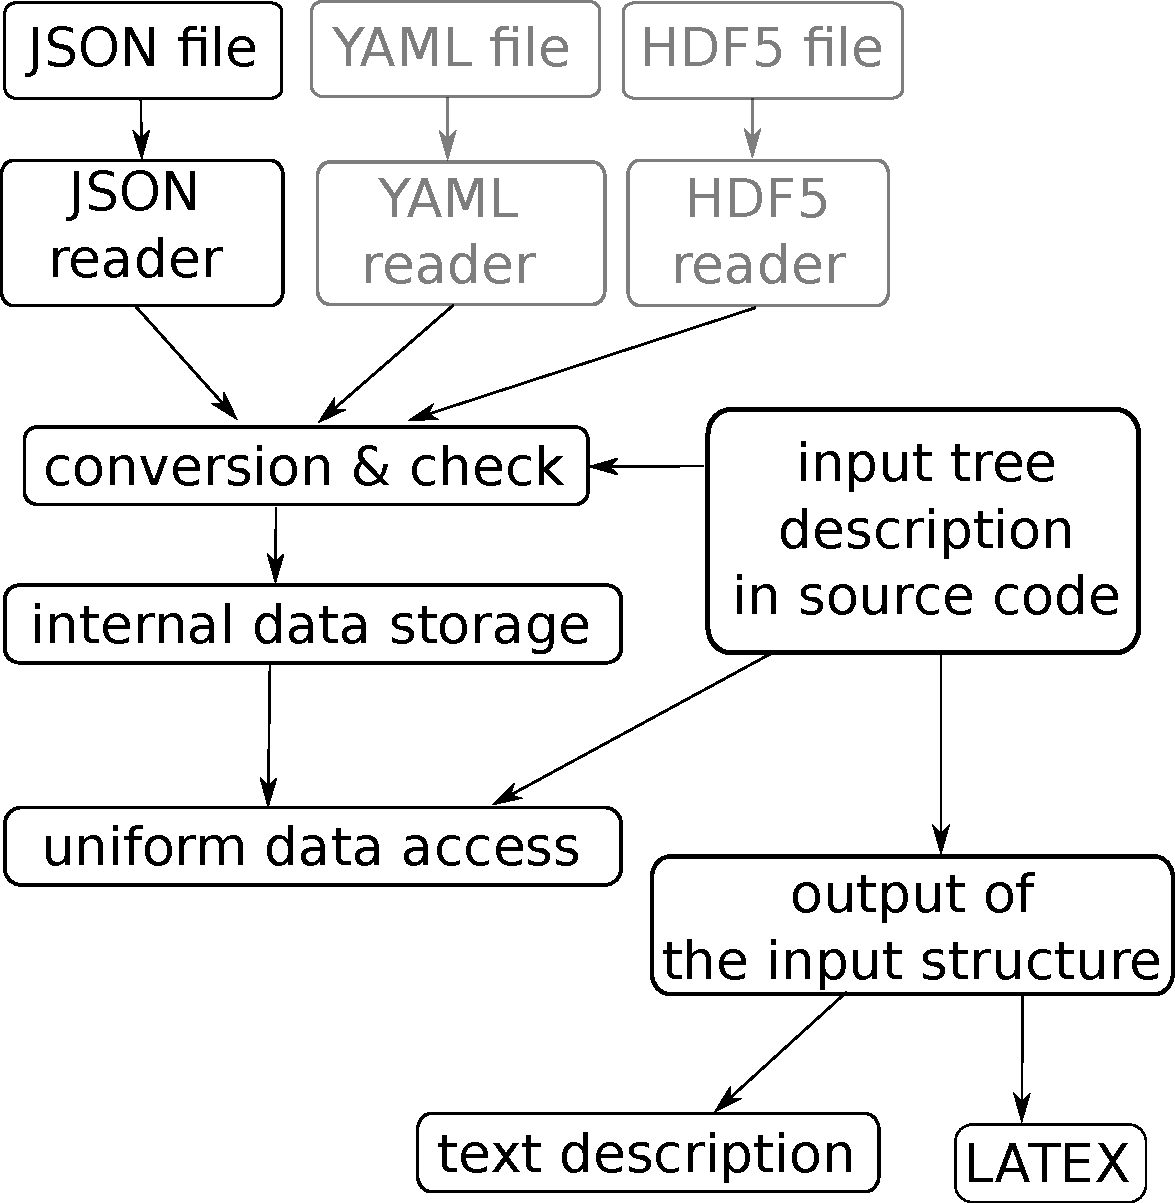
\includegraphics[scale=0.4]{\fig/input_subsystem.pdf}
 % input_subsystem.pdf: 0x0 pixel, -2147483648dpi, 0.00x0.00 cm, bb=
 \caption{Sturucture of the input subsystem. Grey boxes are not implemented yet.}
 \label{fig:input_subsystem}
 \end{center}
\end{figure}

In this section, we shall describe structure of the main input file that is given through the parameter \verb'-s' on the command line.
The file formats of other files that are referenced from the main input file and used for input of the mesh or large field data
(e.g. the GMSH file format) are described in following sections. The input subsystem was designed with the aim to provide uniform initialization of 
C++ classes and data structures. Its structure is depicted on Figure \ref{fig:input_subsystem}.
The structure of the input is described by the Input Types Tree (ITT) of (usually static) objects which follows the structure of the classes.
The data from an input file are read by apropriate reader, their structure is checked against ITT and they are pushed into the Internal Storage Buffer (ISB).
An accessor object to the root data record is the result of the file reading. The data can be retrieved through accessors which combine 
raw data stored in in IBS with their meaning described in ITT. ITT can be printed out in various formats providing description of the input structure both for 
humans and other software.

Currently, the JSON input file format is only implemented and in fact it is slight extension of the JSON file format. On the other hand
the data for initialization of the C++ data structures are coded in particular way. Combination of this extension and restriction of the JSON file format produce 
what we call CON (C++ object notation) file format.


\subsection{JSON for Humans}

Basic syntax of the CON file is very close to the JSON file format with only few extensions, namely:
\begin{itemize}
\item You can use C++ (or JavaScript) comments. One line comments \verb'//' and multi-line comments \verb'/* */'.
\item The quoting of the keys is optional if they do not contain spaces (holds for all CON keys).
\item You can use equality sign \verb'=' instead of colon \verb':' for separation of keys and values in JSON objects.
\item You can use any whitespace to separate tokens in JSON object or JSON array.
\end{itemize}
The aim of these extensions is to simplify writing input files manually. However these extensions can be easily filtered out and converted to 
the generic JSON format. For the description of the JSON format we refer to \url{http://www.json.org/}. 

\subsection{CON Constructs}
The CON file format constructs are designed for initialization of C++ strongly typed variables. The primitive data types can be initialized from 
the primitive CON constructs: 
\begin{itemize}
 \item {\it Bool} --- initialized from the JSON keywords \verb'true' and \verb'false'.
 \item {\it Double}, {\it Integer} --- initialized from JSON numeric data. 
 \item {\it String}, {\it FileName}, {\it Selections} --- initialized from JSON strings
\end{itemize}
Selections are typed like the C++ enum types that are initialized from them.
Various kind of containers can be initialized by the {\it Array} construct, that is an JSON array with elements of the same CON type. 
The C++ structures and classes can be initialize from the {\it Record} construct, which is represented by a JSON object. However, in constrast to JSON,
these Records have different types in similar way as the strong typed C++ structures. The types are described by ITT of the particular program
which can be printed out in several formats, in particular description of ITT for Flow123d forms content of Chapter \ref{chapter:input-tree-reference}.
In order to allow certain kind of polymorphism, we introduce also the {\it AbstractRecord} construct, where the type of the record is not given by ITT but 
can be chosen as part of the input. 

\subsection{CON Special Keys}
All keys in Records should be in lower case, possibly using digits and underscore. The keys all in upper case are reserved for special function in the 
CON file. These are:
\begin{description}

\item[TYPE key]:
\begin{verbatim}
TYPE=<Selection of AbstractRecord>
\end{verbatim}
Is used to specify particular type of an AbstractRecord. This way you can choose which particular implementation of an abstract C++ class should be instantiated.
The value of the key is a string from the Selection that consists of names of Records that was declared as descendants of the AbstractRecord.


%\item[INCLUDE\_RECORD]:\\
%This is a simple inclusion of another file as a content of a record:
%\begin{verbatim}
%{
%        INCLUDE_RECORD = "<file name>"
%}
%\end{verbatim}
%
%\item[INCLUDE\_ARRAY]:\\
%\begin{verbatim}
%array=
%{
%        INCLUDE_ARRAY = "<file name>"
%        FORMAT = "<format string>"
%}       
%\end{verbatim}
%The reader will substitute the include record by a sequentially accessible array. The file has fixed number of 
%space separated data fields on every line. Every line becomes one element in the array of type record. Every line forms a 
%record with key names given by the \verb'<format string>' 
%and corresponding data taken form the line.

%The key difference compared to regular JSON arrays is that included arrays can be accessed only sequentially 
%within the program and thus we minimize reader memory overhead for large input data. The idea is to translate raw data into structured
%format and use uniform access to the data.

%Basic syntax for format string could be an array of strings --- formats of individual columns.
%Every format string is an address of key that is given the column. Onother possibility is to give an arbitrary 
%JSON file, where all values are numbers of columns where to take the value.

%[\dots better specify format string]


%Possible extensions:
% have sections in the file for setting time dependent data
% have number of lines at the beginning
% have variable format
% allow vectors in the 'line records']

\item[REF key]:
\begin{verbatim}
{ REF=<address> }
\end{verbatim}
The record in input file that contains only the key \verb'REF' is replaced by the JSON entity that is referenced by the \verb'<address>'. 
The address is a string with format similar to UNIX path, i.e. with grammar
\begin{verbatim}
    <address> = <address> / <item>
              = <item>  
              = <null>
    <item> = <index>
           = <key>
           = ..
\end{verbatim}
where \verb'index' is non-negative integer and key is valid CON record key (lowercase, digits, underscores).
The address can be absolute or relative identification of an entity. The relative address is relative to the entity in which the reference record is contained.
One can use two dots \verb'".."' to move to parent entity.

Example:
\begin{verbatim}
mesh={
        file_name="xyz"
}
array=[
        {x=1 y=0}       
        {x=2 y=0}
        {x=3 y=0}
]               
outer_record={
        output_file="x_out"
        inner_record={
                output_file={REF="../output_file"} // value "x_out"
        }
        x={REF="/array/2/x"}                       // value "3"
        f_name={REF="/mesh/file_name"}             // value "xyz"
}       
\end{verbatim}
\end{description}

\subsection{Record Types}
A Record type is given by the set of key specifications, which in turn consist from: key name, type of value and default value specification.
Default value specification can be:
\begin{description} 
 \item[obligatory] --- means no default value, which has to be specified at input. 
 \item[optional] --- means no default value, but value is needs not to be specified. Unspecified value usually means that you turn off some functionality.
 \item[default at declaration] --- the default value is explicitly given in declaration and is automatically provided by the input subsystem if needed
 \item[default at read time] --- the default value is provided at read time, usually from some other variable. In the documentation, 
 there is only textual description where the default value comes from.
\end{description}

\subsubsection{Implicit Creation of Composed Entities}
Consider a Record type in which all keys have default values (possibly except one). Then the specification
of the Record can contain a {\it key for default construction}. User can specify only the value of this particular key instead of the whole record, all other keys are initialized from its default values.
Moreover, an AbstractRecord type may have a default value for the \verb'TYPE' key.
This allows to express simple tasks by simple inputs but still make complex inputs possible. 
Similar functionality holds for arrays. If the user sets a non-array value where an array is expected the reader provides an array with a unique element holding the given value.


\section{Important Record Types of Flow123d Input}


\subsection{Mesh Record}
\label{sec:Mesh}
The \hyperlink{IT::Mesh}{mesh record} provides initialization for the computational mesh consisting of points, lines, triangles and tetrahedrons in 3D space.
Currently, we support only GMSH mesh file format \href{http://geuz.org/gmsh/doc/texinfo/gmsh.html#MSH-ASCII-file-format}{MSH ASCII}. 
The input file is provided by the key \hyperA{Mesh::mesh-file}{{\tt mesh\_file}}. The file format allows to group elements into {\it regions} identified either by ID number or by string label. 
The regions with labels starting with the dot character are treated as {\it boundary regions}. Their elements are removed from the computational domain, however they can be used to specify boundary
conditions. Other regions are called {\it bulk regions}. User can create new labeled regions through the key 
\hyperA{Mesh::regions}{{\tt regions}}, the new region can be specified either by its ID
or by list of IDs of its elements. The latter possibility overrides original region assigned to the elements, which can be useful for specification of small areas ``ad hoc''.
The key \hyperA{Mesh::sets}{{\tt sets}} allows specification of sets of regions in terms of list of region IDs or labels and basic set operations. The difference between regions and sets is that
regions form disjoint covering of elements, the sets, however, may overlap. There are three predefined region sets: ``ALL'', ``BOUNDARY'', ``BULK''.


\subsection{Field Records}
\label{sec:Fields}
A general time and space dependent, scalar, vector, or  tensor valued function can be specified through the family of abstract records 
Field $R^m -> \mathcal{S}$, where $m$ is currently always $m=3$ and $\mathcal{S}$ is a specification of the target space, which can be:
\begin{itemize}
 \item {\bf $\mathcal{T}$} --- scalar valued field, with scalars of type $\mathcal{T}$
 \item {\bf $\mathcal{T}[d]$} --- vector valued field, with vector of fixed size $d$ and elements of type $\mathcal{T}$
 \item {\bf $\mathcal{T}[\tt n]$} --- vector valued field, with vector of variable size (given by some input) and elements of type $\mathcal{T}$
 \item {\bf $\mathcal{T}[d, d]$} --- tensor valued field, with square tensor of fixed size and elements of type $\mathcal{T}$
\end{itemize}
the scalar types can be
\begin{itemize}
 \item {\bf Real} --- scalar real valued field
 \item {\bf Int}  --- scalar integer valued field
 \item {\bf Enum} --- scalar non negative integer valued field, should be convertible to appropriate C++ enum type
\end{itemize}

Each of these abstract record has the same set of descendants which implement various algorithms to specify and compute values of the field. These are
\begin{description}
 \item[FieldConstant] --- field that is constant in space
 \item[FieldFormula] --- field that is given by runtime parsed formula using $x,y,z,t$ coordinates. The \href{http://warp.povusers.org/FunctionParser/}{Function Parser} library is used
 with syntax rules described \href{http://warp.povusers.org/FunctionParser/fparser.html#literals}{here}.
 \item[FieldPython] --- field can be implemented by Python script either specified by string (key \hyperA{FieldPython::script-string}{{\tt script\_string}}) 
 or in external file (key \hyperA{FieldPython::script-file}{{\tt script\_file}}. 
 \item[FieldElementwise] --- discrete field, currently only piecewise constant field on elements is supported, the field can given by 
 the \href{http://geuz.org/gmsh/doc/texinfo/gmsh.html#MSH-ASCII-file-format}{MSH ASCII} file specified in key \hyperA{FieldElementwise::gmsh-file}{{\tt gmsh\_file}} and field name in the file given 
 by key \hyperA{FieldElementwise::field-name}{{\tt field\_name}}. The file must contain same mesh as is used for computation.
 \item[FieldInterpolated] --- allows interpolation between different meshes. Not yet fully supported.
\end{description}

Several automatic conversions are implemented. Scalar values can be used to set constant vectors or tensors. Vector value of size $d$ can be used to set diagonal tensor $d\times d$.
Vector value of size $d(d-1)/2$, e.g. $6$ for $d=3$, can be used to set symmetric tensor. These rules apply only for FieldConstant and FieldFormula.
Moreover, all Field abstract types have default value \verb'TYPE=FieldConstant'. Thus you can just use the constant value instead of the whole record.

Examples:
\begin{verbatim}
constant_scalar_function = 1.0
// is same as
constant_scalar_function = {
  TYPE=FieldConstant,
  value=1.0
}

conductivity_tensor = [1 ,2, 3]
// is same as
conductivity_tensor = {
    TYPE=FieldConstant,
    value=[[1,0,0],[0,2,0],[0,0,3]]
}

concentration = {
    TYPE=FieldFormula,
    value="x+y+z"
}
//is same as (provided the vector has 2 elements)
concentration = {
    TYPE=FieldFormula,
    value=["x+y+z", "x+y+z"]
}       
\end{verbatim}

\subsection{Field Data for Equations}
Every equation record has key \verb'input_fields', intended to set both the bulk and boundary fields. These keys contain an array of region-time initialization records
like the \hyperlink{IT::DarcyFlowMH-Data}{\tt Data} record of the DarcyFlow equation. Every such record specifies fields on particular region 
(keys \hyperA{DarcyFlowMH-Steady-BulkData::region}{{\tt region}} and \hyperA{DarcyFlowMH-Steady-BulkData::rid}{{\tt rid}} ) or on a region set 
(key \hyperA{DarcyFlowMH-Steady-BulkData::r-set}{{\tt r\_set}}) starting from the time specified by the key \hyperA{DarcyFlowMH-Steady-BulkData::time}{{\tt time}}.
The array is processed sequentially and latter values overwrite the previous ones. Times should form a non-decreasing sequence.

Example:
\begin{verbatim}
input_fields = [   
    { // time=0.0  - default value
        r_set="BULK",
        conductivity=1   // setting the conductivity field on all regions
    },
    {
        region="2d_part",
        conductivity=2  // overwriting the previous value
    },
    {   time=1.0,
        region="2d_part",
        conductivity={
            // from time=1.0 we switch to the linear function in time
            TYPE=FieldFormula,
            value="2+t"      
        }    
    },
    {   time=2.0,
        region="2d_part",
        conductivity={
            // from time=2.0 we switch to elementwise field, but only
            // on the region "2d_part"
            TYPE=FieldElementwise,
            gmsh_file="./input/data.msh",
            field_name="conductivity"
        }
    }    
]               
\end{verbatim}



% % Copyright (C) 2007 Technical University of Liberec.  All rights reserved.
%
% Please make a following refer to Flow123d on your project site if you use the program for any purpose,
% especially for academic research:
% Flow123d, Research Centre: Advanced Remedial Technologies, Technical University of Liberec, Czech Republic
%
% This program is free software; you can redistribute it and/or modify it under the terms
% of the GNU General Public License version 3 as published by the Free Software Foundation.
%
% This program is distributed in the hope that it will be useful, but WITHOUT ANY WARRANTY;
% without even the implied warranty of MERCHANTABILITY or FITNESS FOR A PARTICULAR PURPOSE.
% See the GNU General Public License for more details.
%
% You should have received a copy of the GNU General Public License along with this program; if not,
% write to the Free Software Foundation, Inc., 59 Temple Place - Suite 330, Boston, MA 021110-1307, USA.


\section{Mesh and Data File Format MSH ASCII}
\label{mesh_file}

Currently, the only supported format for the computational mesh is MSH ASCII format used
by the GMSH software. You can find its documentation on:

\url{http://geuz.org/gmsh/doc/texinfo/gmsh.html#MSH-ASCII-file-format}

The scheme of the file is as follows:
\begin{verbatim}
$MeshFormat
<format version>
$EndMeshFormat

$PhysicalNames
<number of items>
<dimension>     <region ID>     <region label>
...
$EndPhysicalNames

$Nodes
<number of nodes>
<node ID> <X coord> <Y coord> <Z coord>
...
$EndNodes

$Elements
<number of elements>
<element ID> <element shape> <n of tags> <tags> <nodes>
...
$EndElements

$ElementData
<n of string tags>
    <field name>
    <interpolation scheme>
<n of double tags>
    <time>
<n of integer tags>
    <time step index>
    <n of components>
    <n of items>
    <partition index>
<element ID> <component 1> <component 2> ...
...
$EndElementData
\end{verbatim}
Detailed description of individual sections:
\begin{description}
 \item[{\tt PhysicalNames}] : Assign labels to region IDs. Elements of one region should have common dimension. 
    Flow123d interprets regions with labels starting with period as the boundary elements that are not used for calculations.
 \item[{\tt Nodes}] : {\tt <number of nodes>} is also number of data lines that follows. 
    Node IDs are unique but need not to form an aritmetic sequance. Coordinates are float numbers.
 \item[{\tt Elements}] : Element IDs are unique but need not to form an aritmetic sequence. 
    Integer code {\tt <element shape>} represents the shape of element, we support only points (15), lines (1), triangles (2), and tetrahedrons (4).
    Default number of tags is 3. The first is the region ID, the second is ID of the geometrical entity (that was used in original geometry file from which the mesh was generated),
    and the third tag is the partition number. {\tt nodes} is list of node IDs with size according to the element shape.
 \item[{\tt ElementData}] : The header has 2 string tags, 1 double tag, and 4 integer tags with default meaning. For the purpose of the \verb'FieldElementwise' the tags
    \verb'<field name>', \verb'<n of components>', and \verb'<n of items>' are obligatory. This header is folowed by field data on individual elements. 
    Flow123d assumes that elements are sorted by {\tt element ID}, but doesn't need to form a continuos sequence.
\end{description}


%%%%%%%%%%%%%%%%%%%%%%%%%%%%%%%%%%%%%%%%%%%%%%%%%%%%%%%%%%%%%%%%%%%%%%%%%%%%%%%%%%%%%%%%%%%%%


% % Copyright (C) 2007 Technical University of Liberec.  All rights reserved.
%
% Please make a following refer to Flow123d on your project site if you use the program for any purpose,
% especially for academic research:
% Flow123d, Research Centre: Advanced Remedial Technologies, Technical University of Liberec, Czech Republic
%
% This program is free software; you can redistribute it and/or modify it under the terms
% of the GNU General Public License version 3 as published by the Free Software Foundation.
%
% This program is distributed in the hope that it will be useful, but WITHOUT ANY WARRANTY;
% without even the implied warranty of MERCHANTABILITY or FITNESS FOR A PARTICULAR PURPOSE.
% See the GNU General Public License for more details.
%
% You should have received a copy of the GNU General Public License along with this program; if not,
% write to the Free Software Foundation, Inc., 59 Temple Place - Suite 330, Boston, MA 021110-1307, USA.

\section{Output Files}
\label{section_output}

Flow123d supports output of scalar, vector and tensor data fields into two formats. The first is the native format of the GMSH software (usually with extension \verb'msh')
which contains computational mesh followed by data fields for sequence of time levels. The second is the XML version of VTK files. These files can be 
viewed and post-processed by several visualization software packages. However, our primal goal is to support data transfer into the Paraview visualization software.
See key \hyperA{OutputStream::format}{{\tt format}}.

Input record of every equation (flow, transport, reactions, heat) contains the keys {\tt output\_stream} and {\tt output\_fields}.
In {\tt output\_stream}, the name and type of the output file is specified.
Further, in {\tt output\_fields}, one determines the list of fields intended for output.
The available output fields include input data as well as the simulation results.

Below we mention the most important output fields of all equations and link to the complete lists.

\begin{tabular}{|l|p{10cm}|}
\hline
\multicolumn{2}{|l|}{\bf Darcy flow}\\
\hline
\tt pressure\_p0 & Pressure head \units{}{1}{}, piecewise constant on every element. This field is directly produced by the MH method and thus contains no postprocessing error. \\
\hline
\tt pressure\_p1 & Same pressure head field, but interpolated into $P1$ continuous scalar field. Namely you lost dicontinuities on fractures.\\
\hline
\tt velocity\_p0 & Vector field of water flux \units{}{3}{-1}. For every element we evaluate discrete flux field in barycenter.\\
\hline
\tt piezo\_head\_p0 & Piezometric head \units{}{1}{}, piecewise constant on every element. This is just pressure on element  plus z-coordinate of the barycenter. This field is produced only on demand
 (see key \hyperlink{IT::DarcyMHOutput-Selection}{\tt piezo\_head\_p0}).\\
 \hline
complete list & See \hyperlink{IT::DarcyMHOutput-Selection}{Darcy flow output fields}.\\
\hline
% \end{tabular}
% 
% \begin{tabular}{|l|p{10cm}|}
% \hline
\multicolumn{2}{|l|}{\bf Convection transport}\\
\hline
\tt conc & Concentration \units{1}{-3}{}, piecewise constant on every element.\\
 \hline
complete list & See \hyperlink{IT::ConvectionTransport-Output}{Convection transport output fields}.\\
\hline
% \end{tabular}
% 
% \begin{tabular}{|l|p{10cm}|}
% \hline
\multicolumn{2}{|l|}{\bf Transport with dispersion}\\
\hline
\tt conc & Concentration \units{1}{-3}{}, piecewise linear on every element. Even if higher order polynomial approximation is used in simulation, the results are saved only in element corners.\\
 \hline
complete list & See \hyperlink{IT::SoluteTransport-DG-Output}{Transport with dispersion output fields}.\\
\hline
% \end{tabular}
% 
% \begin{tabular}{|l|p{10cm}|}
% \hline
\multicolumn{2}{|l|}{\bf Dual porosity}\\
\hline
\tt conc\_immobile & Concentration \units{1}{-3}{} in immobile zone, piecewise linear on every element.\\
 \hline
complete list & See \hyperlink{IT::DualPorosity-Output}{Dual porosity output fields}.\\
\hline
% 
\multicolumn{2}{|l|}{\bf Sorption, Mobile sorption, Immobile sorption}\\
\hline
\tt conc\_solid & Concentration [mol\,$\mathrm{kg}^{-1}$] of sorbed substance, piecewise linear on every element.\\
 \hline
complete list & See \hyperlink{IT::Sorption-Output}{Sorption output fields}, \hyperlink{IT::SorptionMobile-Output}{Mobile sorption output fields}, \hyperlink{IT::SorptionImmobile-Output}{Immobile sorption output fields}.\\
\hline
% 
\multicolumn{2}{|l|}{\bf Heat transfer}\\
\hline
\tt temperature & Temperature [K], piecewise linear on every element. Even if higher order polynomial approximation is used in simulation, the results are saved only in element corners.\\
 \hline
complete list & See \hyperlink{IT::HeatTransfer-DG-Output}{Heat transfer output fields}.\\
\hline
\end{tabular}




% \subsection{Output data fields of water flow module}
% Water flow module provides output of four data fields. 
% \begin{description}
%  \item[pressure on elements] Pressure head in length units $[L]$ piecewise constant on every element. This field is directly produced by the MH method and thus contains no postprocessing error.
%  \item[pressure in nodes] Same pressure head field, but interpolated into $P1$ continuous scalar field. Namely you lost dicontinuities on fractures.
%  \item[velocity on elements] Vector field of water flux volume unit per time unit $[L^3 / T]$. For every element we evaluate discrete flux field in barycenter.
%  \item[piezometric head on elements] Piezometric head in length units $[L]$ piecewise constant on every element. This is just pressure on element  plus z-coordinate of the barycenter. This field is produced only on demand
%  (see key \hyperA{DarcyMHOutput::piezo-head-p0}{\tt piezo\_head\_p0}).
% \end{description}
% 
% \subsection{Output data fields of transport}
% Transport module provides output only for concentrations (in mobile phase) as a field piecewise constant over elements. There is one field for every substance and names of those fields contain 
% names of substances given by key \hyperA{TransportOperatorSplitting::substances}{{\tt substances}}. The physical unit is mass unit over volume unit $[M / L^3]$.



%\subsection{GMSH viewer remarks}

%\subsection{Paraview viewer remarks}

\subsection{Auxiliary Output Files}

\subsubsection{Profiling Information}
On every run we collect some basic profiling informations. After all computations these data are written into the file
\verb'profiler%y%m%d_%H.%M.%S.out' where \verb'%y', \verb'%m', \verb'%d', \verb'%H', \verb'%M', \verb'%S' are 
two digit numbers representing year, month, day, hour, minute, and second of the program start time.

\subsubsection{Balance of Conservative Quantities}
Primary and secondary equations can produce additional information on fluxes, sources and state of conservative quantities (for flow it is the volume of water, for transport the mass of a substance, for heat transfer the energy).
The computation of balance is governed by the key \verb'balance'.
The balance file (default \verb'water_balance.txt', \verb'mass_balance.txt', \verb'energy_balance.txt') contains the following information:
\begin{itemize}
\item time and region
\item name and unit of the quantity
\item mass (current state), flux through boundary and volume source at given time and region
\item incoming and outgoing flux and source
\item flux and source increment since the last balance output time
\item cumulative flux and source
\item error: current mass should equal to initial mass + cumulative sources - cumulative fluxes
\end{itemize}


\subsubsection{Raw Water Flow Data File}
You can force Flow123d to write raw data about results of MH method. The file format is:
\begin{verbatim}
$FlowField
T=<time>
<number fo elements>
<eid> <pressure> <flux x> <flux y> <flux z> <number of sides> <pressures on sides> <fluxes on sides> 
...
$EndFlowField
\end{verbatim}

where 
\begin{description}
 \item \verb'<time>' --- is simulation time of the raw output.
 \item \verb'<number of elements>' --- is number of elements in mesh, which is same as number of subsequent lines.
 \item \verb'<eid>' --- element id same as in the input mesh.
 \item \verb'<flux x,y,z>' --- components of water flux interpolated to barycenter of the element
 \item \verb'<number of sides>' --- number of sides of the element, infulence number of remaining values
 \item \verb'<pressures on sides>' --- for every side average of the pressure over the side
 \item \verb'<fluxes on sides>' --- for ever side total flux through the side 
\end{description}


% %\input{tso_10} 
% %\input{pos_12}   

% % TODO: Update description of tests
% % \chapter{Test and tutorial problems (WORK IN PROGRESS)}
% %  \label{chapter:tests}
% %  \input{tests}
% % 
% %  \chapter{Comparision of versions (WORK IN PROGRESS)}
% %  \label{chapter:version_comparision}
% %  \input{version_comparision}

% \chapter{Main Input File Reference}
% \label{chapter:input-tree-reference}
% support macros

% generated file
\begin{RecordType}{\hyperB{IT::SequentialCoupling}{SequentialCoupling}}{\Alink{IT::Problem}{Problem}}{}{}{Record with data for a general sequential coupling.
}
\KeyItem{\hyperB{SequentialCoupling::TYPE}{TYPE}} <<Missing formatter for <class 'ist.nodes.Selection'>>>
\KeyItem{\hyperB{SequentialCoupling::description}{description}}{String (generic)}{\textlangle{\it optional }\textrangle}{}{Short description of the solved problem.
Is displayed in the main log, and possibly in other text output files.}
\KeyItem{\hyperB{SequentialCoupling::mesh}{mesh}}{record: \Alink{IT::Mesh}{Mesh}}{\textlangle{\it obligatory }\textrangle}{}{Computational mesh common to all equations.}
\KeyItem{\hyperB{SequentialCoupling::time}{time}}{record: \Alink{IT::TimeGovernor}{TimeGovernor}}{\textlangle{\it optional }\textrangle}{}{Simulation time frame and time step.}
\KeyItem{\hyperB{SequentialCoupling::primary-equation}{primary\_equation}}{abstract type: \Alink{IT::DarcyFlowMH}{DarcyFlowMH}}{\textlangle{\it obligatory }\textrangle}{}{Primary equation, have all data given.}
\KeyItem{\hyperB{SequentialCoupling::secondary-equation}{secondary\_equation}}{abstract type: \Alink{IT::Transport}{Transport}}{\textlangle{\it optional }\textrangle}{}{The equation that depends (the velocity field) on the result of the primary equation.}
\end{RecordType}


\bibliographystyle{abbrvnat}
\bibliography{flow123d_doc.bib}
%%%%%%%%%%%%%%%%%%%%%%%%%%%%%%%%%%%%%%%%%%%%%%%%%%%%%%%%%%%%%%%%%%%%%%%%%%%%%%%%%%%%%%%%%%%%%%%%%%%%%%%%%%%%%%%%%


\end{document}


